\documentclass{article}

\usepackage{arxiv}

\usepackage[utf8]{inputenc} % allow utf-8 input
\usepackage[T1]{fontenc}    % use 8-bit T1 fonts
\usepackage{lmodern}        % https://github.com/rstudio/rticles/issues/343
\usepackage{hyperref}       % hyperlinks
\usepackage{url}            % simple URL typesetting
\usepackage{booktabs}       % professional-quality tables
\usepackage{amsfonts}       % blackboard math symbols
\usepackage{nicefrac}       % compact symbols for 1/2, etc.
\usepackage{microtype}      % microtypography
\usepackage{lipsum}
\usepackage{graphicx}

\title{Volatility and Spillover: Facts of Market Life}

\author{
    William G. Foote
    \thanks{Thanks to numberous colleagues and financial engineering
students at Manhattan College and Syracuse University for the organic
development of the ideas in this paper.}
   \\
    Department of Business Analytics \\
    Manhattan College \\
  Riverdale, NY 10471 \\
  \texttt{\href{mailto:wfoote01@manhattan.edu}{\nolinkurl{wfoote01@manhattan.edu}}} \\
   \And
    Brian Wholey
   \\
    Manhattan College \\
  Riverdale, NY 10471 \\
  \texttt{\href{mailto:bwholey01@manhattan.edu}{\nolinkurl{bwholey01@manhattan.edu}}} \\
  }

\usepackage{color}
\usepackage{fancyvrb}
\newcommand{\VerbBar}{|}
\newcommand{\VERB}{\Verb[commandchars=\\\{\}]}
\DefineVerbatimEnvironment{Highlighting}{Verbatim}{commandchars=\\\{\}}
% Add ',fontsize=\small' for more characters per line
\usepackage{framed}
\definecolor{shadecolor}{RGB}{248,248,248}
\newenvironment{Shaded}{\begin{snugshade}}{\end{snugshade}}
\newcommand{\AlertTok}[1]{\textcolor[rgb]{0.94,0.16,0.16}{#1}}
\newcommand{\AnnotationTok}[1]{\textcolor[rgb]{0.56,0.35,0.01}{\textbf{\textit{#1}}}}
\newcommand{\AttributeTok}[1]{\textcolor[rgb]{0.77,0.63,0.00}{#1}}
\newcommand{\BaseNTok}[1]{\textcolor[rgb]{0.00,0.00,0.81}{#1}}
\newcommand{\BuiltInTok}[1]{#1}
\newcommand{\CharTok}[1]{\textcolor[rgb]{0.31,0.60,0.02}{#1}}
\newcommand{\CommentTok}[1]{\textcolor[rgb]{0.56,0.35,0.01}{\textit{#1}}}
\newcommand{\CommentVarTok}[1]{\textcolor[rgb]{0.56,0.35,0.01}{\textbf{\textit{#1}}}}
\newcommand{\ConstantTok}[1]{\textcolor[rgb]{0.00,0.00,0.00}{#1}}
\newcommand{\ControlFlowTok}[1]{\textcolor[rgb]{0.13,0.29,0.53}{\textbf{#1}}}
\newcommand{\DataTypeTok}[1]{\textcolor[rgb]{0.13,0.29,0.53}{#1}}
\newcommand{\DecValTok}[1]{\textcolor[rgb]{0.00,0.00,0.81}{#1}}
\newcommand{\DocumentationTok}[1]{\textcolor[rgb]{0.56,0.35,0.01}{\textbf{\textit{#1}}}}
\newcommand{\ErrorTok}[1]{\textcolor[rgb]{0.64,0.00,0.00}{\textbf{#1}}}
\newcommand{\ExtensionTok}[1]{#1}
\newcommand{\FloatTok}[1]{\textcolor[rgb]{0.00,0.00,0.81}{#1}}
\newcommand{\FunctionTok}[1]{\textcolor[rgb]{0.00,0.00,0.00}{#1}}
\newcommand{\ImportTok}[1]{#1}
\newcommand{\InformationTok}[1]{\textcolor[rgb]{0.56,0.35,0.01}{\textbf{\textit{#1}}}}
\newcommand{\KeywordTok}[1]{\textcolor[rgb]{0.13,0.29,0.53}{\textbf{#1}}}
\newcommand{\NormalTok}[1]{#1}
\newcommand{\OperatorTok}[1]{\textcolor[rgb]{0.81,0.36,0.00}{\textbf{#1}}}
\newcommand{\OtherTok}[1]{\textcolor[rgb]{0.56,0.35,0.01}{#1}}
\newcommand{\PreprocessorTok}[1]{\textcolor[rgb]{0.56,0.35,0.01}{\textit{#1}}}
\newcommand{\RegionMarkerTok}[1]{#1}
\newcommand{\SpecialCharTok}[1]{\textcolor[rgb]{0.00,0.00,0.00}{#1}}
\newcommand{\SpecialStringTok}[1]{\textcolor[rgb]{0.31,0.60,0.02}{#1}}
\newcommand{\StringTok}[1]{\textcolor[rgb]{0.31,0.60,0.02}{#1}}
\newcommand{\VariableTok}[1]{\textcolor[rgb]{0.00,0.00,0.00}{#1}}
\newcommand{\VerbatimStringTok}[1]{\textcolor[rgb]{0.31,0.60,0.02}{#1}}
\newcommand{\WarningTok}[1]{\textcolor[rgb]{0.56,0.35,0.01}{\textbf{\textit{#1}}}}

% Pandoc citation processing
\newlength{\csllabelwidth}
\setlength{\csllabelwidth}{3em}
\newlength{\cslhangindent}
\setlength{\cslhangindent}{1.5em}
% for Pandoc 2.8 to 2.10.1
\newenvironment{cslreferences}%
  {}%
  {\par}
% For Pandoc 2.11+
\newenvironment{CSLReferences}[2] % #1 hanging-ident, #2 entry spacing
 {% don't indent paragraphs
  \setlength{\parindent}{0pt}
  % turn on hanging indent if param 1 is 1
  \ifodd #1 \everypar{\setlength{\hangindent}{\cslhangindent}}\ignorespaces\fi
  % set entry spacing
  \ifnum #2 > 0
  \setlength{\parskip}{#2\baselineskip}
  \fi
 }%
 {}
\usepackage{calc} % for calculating minipage widths
\newcommand{\CSLBlock}[1]{#1\hfill\break}
\newcommand{\CSLLeftMargin}[1]{\parbox[t]{\csllabelwidth}{#1}}
\newcommand{\CSLRightInline}[1]{\parbox[t]{\linewidth - \csllabelwidth}{#1}\break}
\newcommand{\CSLIndent}[1]{\hspace{\cslhangindent}#1}

\usepackage{amsmath}


\begin{document}
\maketitle

\def\tightlist{}


\begin{abstract}
Volatility and the interaction of markets continue to beguile traders,
managers, investors and regulators. In this preliminary draft we use a
working example from the renewable energy industry to develop three work
flows for financial time series: univariate empirical characterizations;
quantile regression spillover analysis; and bayesian multi-level
hierarchical generation of a stratified industry risk structure. This
latter flow deploys a Pareto-smoothed importance sampling with
leave-one-out cross-validation to investigate uncertainty and
variability of market events, especially so-called outliers.
\end{abstract}

\keywords{
    market pillover
   \and
    volatility clustering
   \and
    quantile regression
   \and
    bayesian data analysis
   \and
    multi-level hierarchical model
   \and
    pareto-smoothed importance sampling
   \and
    leave-one-out cross validation
  }

\hypertarget{what-are-the-stylized-facts}{%
\section{What are the stylized
facts?}\label{what-are-the-stylized-facts}}

A tool available to financial risk managers is the analysis of market
spillover and volatility clustering. When one market becomes entangled
with another through the normal course of trade, is it possible for the
volatility of one to affect the volatility of another? Theoretically, of
course it is possible. However, the only way to gauge the impact of one
market on another another is through some sort of association analysis,
Here we will use simple linear regression techniques to detect the
existence and degree of market spillover.\footnote{Theory and practice
  are themselves deeply entangled in a dialectical circle. We suppose we
  are naive investors with an account at our favorite online brokerage
  with three assets. We know nothing at the outset but profit and loss.
  We aim to learn a bit more about the three assets starting with their
  history. Our characterization of this history will inform us of the
  deeper reasons why, and how, our profit and loss statements evolve.}

The experience of risk management is that spillover and other market
observations are so common, across multiple market regimes, as to confer
the status of fact. The supposition of such an analysis would be that
managers would ignore such regularly occuring observations to their
detriment. Here is a short compendium of the usual suspects for
univariate series.\footnote{Cont (2001) is generally recognized as the
  first cross asset survey of co-called stylized facts of financial
  markets. McNeil, Frey, and Embrechts (2015) devote Chapter 3 to a
  discussion about the existence of market factors for univariate and
  multivariate financial time series.}

\begin{itemize}
\item
  Risk factor changes exhibit little or no memory, evidenced by
  significant but less impactful dependency on univariate
  autocorrelations at any lag.
\item
  The conditional expectation of returns is nearly always zero.
\item
  On the other hand, volatility of the same series exhibits very slowly
  decaying autocorrelations with power law tail thicknesses.
\item
  Return series are left skewed, while volatility series are naturally
  right skewed but witb persistently thick tails.
\item
  Return series tend to have thick tails with clusters of volatility.
\end{itemize}

This last observation about volatility in practice means that the
conditional standard deviations of returns are themselves volatile.
Volatile volatility is indeed the definition of highly leptokurtotic
returns.\footnote{That is, and much more colloquially, slender tails, to
  translate the original Greek term. But these tails extend to extreme
  values and thus thicken the possibility of occurring far from central
  locations of the data. Taleb (2018) details the use of a very
  different approach to including thick tailed analysis into the
  management of risk.} That the returns cluster reveals a story of the
persistence of high volatility as well as the persistence of low
volatility environments.

On the multivariate front, that is, the portfolio side of the world of
markets we observe these hard to write off facts.\footnote{McNeil, Frey,
  and Embrechts (2015) devote the last half of Chapter 3 to a discussion
  about the existence of market factors for multivariate financial time
  series. Their chapter 7 details three fallacies in the development of
  appropriate, attainable, measures of dependency, of which
  cross-correlation is but one.}

\begin{itemize}
\item
  Returns exhibit little or no non-contemporaneous cross-correlation.
\item
  Volatilities of returns (e.g., absolute values of returns) exhibit
  strong and weakly decaying, thus persistent, cross-correlations.
\item
  Correlations, like volatilities, vary across time.
\item
  Extreme returns on one market invariable relate to extreme returns in
  other markets.
\end{itemize}

It is this very last observation that deserves our attention in this
paper; the experience of market spillover.

\hypertarget{an-initial-work-flow}{%
\section{An initial work flow}\label{an-initial-work-flow}}

We will use the following steps to analyze market spillover.

\begin{enumerate}
\def\labelenumi{\arabic{enumi}.}
\item
  We build and visualize time series objects. We will also convert a
  time series object to a data frame for further processing. Inside of
  this object we will \texttt{summarise()} the data using descriptive
  statistics, estimate and visualize the lagged relationship of current
  and past realizations of the time series, and interpret
  autocorrelation and cross autocorrelation as indications of the styled
  facts of various financial markets.
\item
  We will derive monthly time series of correlations and volatilities
  from daily series.
\item
  We then visualize to analyze the sensitivity of entangled (as measured
  with correlation) markets as an endogenous system of risk.
\item
  We are then in the position to analyze and visualize the impact of one
  market's volatility on another through correlational entanglements
  between markets.
\end{enumerate}

We will also use a probabilistic inference framework, more frequently
called a Bayesian approach, to develop our provisional conclusions. What
we will be able to pull out of the data is the full joint distribution
of cross-market impacts as well as the marginal impacts within each
market, especially as these markets communicate information among
themselves.\footnote{We use the generative stochastic models described
  as Bayesian statistical models in McElreath (2020) coded in R and Stan
  (Carpenter (2017); Team (2020b)) and fit using R (R Core Team) and
  rstan (Team (2020a)). The complete workflow will be maintained on
  GitHub at \url{https://github.com/wgfoote/market-risk}.}

\hypertarget{a-working-example}{%
\section{A working example}\label{a-working-example}}

We suppose that we work with the CFO of an aluminum recycling company.
Here is a story we can use to make practical our insights into connected
markets.

The aluminum recycling company just bought a renewable energy
manufacturing and services company to expand its earnings opportunities.
The renewables devision dabbles in wind, clean energy technologies (very
similar to the aluminum recycling clean technologies), and solar, a very
new field for the company. The CFO would like to measure the impact of
this new market on the earnings of the proposed renewables division. To
do this she commissions a project team.

The CFO has three questions for the team:

\begin{enumerate}
\def\labelenumi{\arabic{enumi}.}
\item
  How do we characterize renewables variability?
\item
  Does one market affect another?
\item
  What stylized facts of these markets matter to the generation of
  earnings in this new division?
\end{enumerate}

For the renewables sector we select
\href{https://www.investopedia.com/terms/e/etf.asp}{exchange traded
funds (ETF)} fromm the
\href{https://www.etf.com/channels/renewable-energy-etfs}{global
renewables sector}: TAN for solar, ICLN for clean technologies, and PBW
for wind.

These funds act as indices to effectively summarize the inputs, process,
management, decisions, and outputs of various aspects of the renewables
sector. Examining and analyzing these series will go a long way to
helping the CFO understand the riskiness of these markets.

Our objective is to review the historical record for volatility and
relationships among three repesentative markets. We load historical data
on the market value of three ETFs, transform prices into returns, and
then further transform the returns into within-month correlations and
standard deviations.

\hypertarget{getting-some-data}{%
\section{Getting some data}\label{getting-some-data}}

We access daily market prices using the \texttt{tidyquant} package and
transform market prices into daily returns and intra-monthly
correlations and standard deviations.

\begin{Shaded}
\begin{Highlighting}[]
\CommentTok{\#}
\FunctionTok{options}\NormalTok{(}\AttributeTok{digits =} \DecValTok{4}\NormalTok{, }\AttributeTok{scipen =} \DecValTok{999999}\NormalTok{)}
\FunctionTok{library}\NormalTok{(ggplot2)}
\FunctionTok{library}\NormalTok{(GGally)}
\FunctionTok{library}\NormalTok{(lubridate)}
\FunctionTok{library}\NormalTok{(dplyr)}
\FunctionTok{library}\NormalTok{(tidyverse)}
\FunctionTok{library}\NormalTok{(quantreg)}
\FunctionTok{library}\NormalTok{(forecast)}
\FunctionTok{library}\NormalTok{(tidyquant)}
\FunctionTok{library}\NormalTok{(timetk)}
\FunctionTok{library}\NormalTok{(quantmod)}
\FunctionTok{library}\NormalTok{(matrixStats)}
\CommentTok{\#}
\NormalTok{symbols }\OtherTok{\textless{}{-}} \FunctionTok{c}\NormalTok{(}\StringTok{"TAN"}\NormalTok{, }\StringTok{"ICLN"}\NormalTok{, }\StringTok{"PBW"}\NormalTok{) }\CommentTok{\#c("ENE", "REP", "")}
\NormalTok{price\_tbl }\OtherTok{\textless{}{-}} \FunctionTok{tq\_get}\NormalTok{(symbols) }\SpecialCharTok{\%\textgreater{}\%} 
  \FunctionTok{select}\NormalTok{(date, symbol, }\AttributeTok{price =}\NormalTok{ adjusted)}
\CommentTok{\# long format ("TIDY") price tibble for possible other work}
\NormalTok{return\_tbl }\OtherTok{\textless{}{-}}\NormalTok{ price\_tbl }\SpecialCharTok{\%\textgreater{}\%} 
  \FunctionTok{group\_by}\NormalTok{(symbol) }\SpecialCharTok{\%\textgreater{}\%} 
  \FunctionTok{tq\_transmute}\NormalTok{(}\AttributeTok{mutate\_fun =}\NormalTok{ periodReturn, }\AttributeTok{period =} \StringTok{"daily"}\NormalTok{, }\AttributeTok{type =} \StringTok{"log"}\NormalTok{, }\AttributeTok{col\_rename =} \StringTok{"daily\_return"}\NormalTok{) }\SpecialCharTok{\%\textgreater{}\%}
  \FunctionTok{mutate}\NormalTok{(}\AttributeTok{abs\_return =} \FunctionTok{abs}\NormalTok{(daily\_return))}
\CommentTok{\#str(return\_tbl)}
\NormalTok{r\_2 }\OtherTok{\textless{}{-}}\NormalTok{ return\_tbl }\SpecialCharTok{\%\textgreater{}\%} 
  \FunctionTok{select}\NormalTok{(symbol, date, daily\_return) }\SpecialCharTok{\%\textgreater{}\%} \FunctionTok{spread}\NormalTok{(symbol, daily\_return)}
\NormalTok{r\_2 }\OtherTok{\textless{}{-}} \FunctionTok{xts}\NormalTok{(r\_2, r\_2}\SpecialCharTok{$}\NormalTok{date)[}\SpecialCharTok{{-}}\DecValTok{1}\NormalTok{, ]}
\FunctionTok{storage.mode}\NormalTok{(r\_2) }\OtherTok{\textless{}{-}} \StringTok{"numeric"}
\NormalTok{r\_2 }\OtherTok{\textless{}{-}}\NormalTok{ r\_2[, }\SpecialCharTok{{-}}\DecValTok{1}\NormalTok{]}
\NormalTok{r\_corr }\OtherTok{\textless{}{-}} \FunctionTok{apply.monthly}\NormalTok{(r\_2, }\AttributeTok{FUN =}\NormalTok{ cor)[,}\FunctionTok{c}\NormalTok{(}\DecValTok{2}\NormalTok{, }\DecValTok{3}\NormalTok{, }\DecValTok{6}\NormalTok{)]}
\FunctionTok{colnames}\NormalTok{(r\_corr) }\OtherTok{\textless{}{-}} \FunctionTok{c}\NormalTok{(}\StringTok{"TAN\_ICLN"}\NormalTok{, }\StringTok{"TAN\_PBW"}\NormalTok{, }\StringTok{"ICLN\_PBW"}\NormalTok{)}
\NormalTok{r\_vols }\OtherTok{\textless{}{-}} \FunctionTok{apply.monthly}\NormalTok{(r\_2, }\AttributeTok{FUN =}\NormalTok{ colSds)}
\CommentTok{\# }
\NormalTok{corr\_tbl }\OtherTok{\textless{}{-}}\NormalTok{ r\_corr }\SpecialCharTok{\%\textgreater{}\%} 
  \FunctionTok{as\_tibble}\NormalTok{() }\SpecialCharTok{\%\textgreater{}\%} 
  \FunctionTok{mutate}\NormalTok{(}\AttributeTok{date =} \FunctionTok{index}\NormalTok{(r\_corr)) }\SpecialCharTok{\%\textgreater{}\%} 
  \FunctionTok{gather}\NormalTok{(}\AttributeTok{key =}\NormalTok{ assets, }\AttributeTok{value =}\NormalTok{ corr, }\SpecialCharTok{{-}}\NormalTok{date)}

\NormalTok{vols\_tbl }\OtherTok{\textless{}{-}}\NormalTok{ r\_vols }\SpecialCharTok{\%\textgreater{}\%} 
  \FunctionTok{as\_tibble}\NormalTok{() }\SpecialCharTok{\%\textgreater{}\%} 
  \FunctionTok{mutate}\NormalTok{(}\AttributeTok{date =} \FunctionTok{index}\NormalTok{(r\_vols)) }\SpecialCharTok{\%\textgreater{}\%} 
  \FunctionTok{gather}\NormalTok{(}\AttributeTok{key =}\NormalTok{ assets, }\AttributeTok{value =}\NormalTok{ vols, }\SpecialCharTok{{-}}\NormalTok{date) }
\CommentTok{\#}
\NormalTok{corr\_vols }\OtherTok{\textless{}{-}} \FunctionTok{merge}\NormalTok{(r\_corr, r\_vols)}
\NormalTok{corr\_vols\_tbl }\OtherTok{\textless{}{-}}\NormalTok{ corr\_vols }\SpecialCharTok{\%\textgreater{}\%} 
  \FunctionTok{as\_tibble}\NormalTok{() }\SpecialCharTok{\%\textgreater{}\%} 
  \FunctionTok{mutate}\NormalTok{(}\AttributeTok{date =} \FunctionTok{index}\NormalTok{(corr\_vols))}
\CommentTok{\#}
\end{Highlighting}
\end{Shaded}

\hypertarget{some-simple-summaries}{%
\subsection{Some simple summaries}\label{some-simple-summaries}}

We use tabular and graphical depictions of the shapes of each of the
correlationa and volatility series. Here is the first routine to
generate a tabular summary of the shape of within-month correlations.

\begin{Shaded}
\begin{Highlighting}[]
\NormalTok{corr\_tbl }\SpecialCharTok{\%\textgreater{}\%} \FunctionTok{group\_by}\NormalTok{(assets) }\SpecialCharTok{\%\textgreater{}\%} 
  \FunctionTok{summarise}\NormalTok{(}\AttributeTok{mean =} \FunctionTok{mean}\NormalTok{(corr), }
            \AttributeTok{sd =} \FunctionTok{sd}\NormalTok{(corr), }\AttributeTok{skew =} \FunctionTok{skewness}\NormalTok{(corr), }
            \AttributeTok{kurt =} \FunctionTok{kurtosis}\NormalTok{(corr), }
            \AttributeTok{min =} \FunctionTok{min}\NormalTok{(corr), }
            \AttributeTok{q\_25 =} \FunctionTok{quantile}\NormalTok{(corr, }\FloatTok{0.25}\NormalTok{), }
            \AttributeTok{q\_50 =} \FunctionTok{quantile}\NormalTok{(corr, }\FloatTok{0.50}\NormalTok{), }
            \AttributeTok{q\_75 =} \FunctionTok{quantile}\NormalTok{(corr, }\FloatTok{0.75}\NormalTok{), }
            \AttributeTok{max =} \FunctionTok{max}\NormalTok{(corr),}
            \AttributeTok{iqr =} \FunctionTok{quantile}\NormalTok{(corr, }\FloatTok{0.75}\NormalTok{) }\SpecialCharTok{{-}} \FunctionTok{quantile}\NormalTok{(corr, }\FloatTok{0.25}\NormalTok{)}
\NormalTok{            )}
\end{Highlighting}
\end{Shaded}

\begin{verbatim}
## # A tibble: 3 x 11
##   assets    mean     sd   skew  kurt   min  q_25  q_50  q_75   max    iqr
##   <chr>    <dbl>  <dbl>  <dbl> <dbl> <dbl> <dbl> <dbl> <dbl> <dbl>  <dbl>
## 1 ICLN_PBW 0.839 0.0974 -1.67  3.55  0.431 0.810 0.854 0.903 0.985 0.0927
## 2 TAN_ICLN 0.719 0.180  -0.839 0.349 0.126 0.597 0.756 0.860 0.982 0.264 
## 3 TAN_PBW  0.790 0.134  -0.793 0.136 0.373 0.703 0.807 0.898 0.981 0.195
\end{verbatim}

We just reuse the code above and substitute \texttt{vols} for
\texttt{corr} to review the volatility data.

\begin{Shaded}
\begin{Highlighting}[]
\NormalTok{vols\_tbl }\SpecialCharTok{\%\textgreater{}\%} \FunctionTok{group\_by}\NormalTok{(assets) }\SpecialCharTok{\%\textgreater{}\%} 
  \FunctionTok{summarise}\NormalTok{(}\AttributeTok{mean =} \FunctionTok{mean}\NormalTok{(vols), }
            \AttributeTok{sd =} \FunctionTok{sd}\NormalTok{(vols), }
            \AttributeTok{skew =} \FunctionTok{skewness}\NormalTok{(vols), }
            \AttributeTok{kurt =} \FunctionTok{kurtosis}\NormalTok{(vols), }
            \AttributeTok{min =} \FunctionTok{min}\NormalTok{(vols), }
            \AttributeTok{q\_25 =} \FunctionTok{quantile}\NormalTok{(vols, }\FloatTok{0.25}\NormalTok{), }
            \AttributeTok{q\_50 =} \FunctionTok{quantile}\NormalTok{(vols, }\FloatTok{0.50}\NormalTok{), }
            \AttributeTok{q\_75 =} \FunctionTok{quantile}\NormalTok{(vols, }\FloatTok{0.75}\NormalTok{), }
            \AttributeTok{max =} \FunctionTok{max}\NormalTok{(vols),}
            \AttributeTok{iqr =} \FunctionTok{quantile}\NormalTok{(vols, }\FloatTok{0.75}\NormalTok{) }\SpecialCharTok{{-}} \FunctionTok{quantile}\NormalTok{(vols, }\FloatTok{0.25}\NormalTok{)}
\NormalTok{            )}
\end{Highlighting}
\end{Shaded}

\begin{verbatim}
## # A tibble: 3 x 11
##   assets   mean      sd  skew  kurt     min    q_25   q_50   q_75    max     iqr
##   <chr>   <dbl>   <dbl> <dbl> <dbl>   <dbl>   <dbl>  <dbl>  <dbl>  <dbl>   <dbl>
## 1 ICLN   0.0142 0.00754  3.42 19.2  0.00519 0.00993 0.0127 0.0166 0.0671 0.00667
## 2 PBW    0.0178 0.00924  2.71 12.3  0.00803 0.0116  0.0158 0.0205 0.0763 0.00887
## 3 TAN    0.0223 0.00975  1.70  6.34 0.00769 0.0150  0.0216 0.0274 0.0758 0.0123
\end{verbatim}

We view densities and line plots of historical correlations with these
routines.

\begin{Shaded}
\begin{Highlighting}[]
\NormalTok{corr\_tbl }\SpecialCharTok{\%\textgreater{}\%} \FunctionTok{ggplot}\NormalTok{(}\FunctionTok{aes}\NormalTok{(}\AttributeTok{x =}\NormalTok{ corr, }\AttributeTok{fill =}\NormalTok{ assets)) }\SpecialCharTok{+} 
  \FunctionTok{geom\_density}\NormalTok{(}\AttributeTok{alpha =} \FloatTok{0.4}\NormalTok{) }\SpecialCharTok{+} 
  \FunctionTok{facet\_wrap}\NormalTok{(}\SpecialCharTok{\textasciitilde{}}\NormalTok{assets)}
\end{Highlighting}
\end{Shaded}

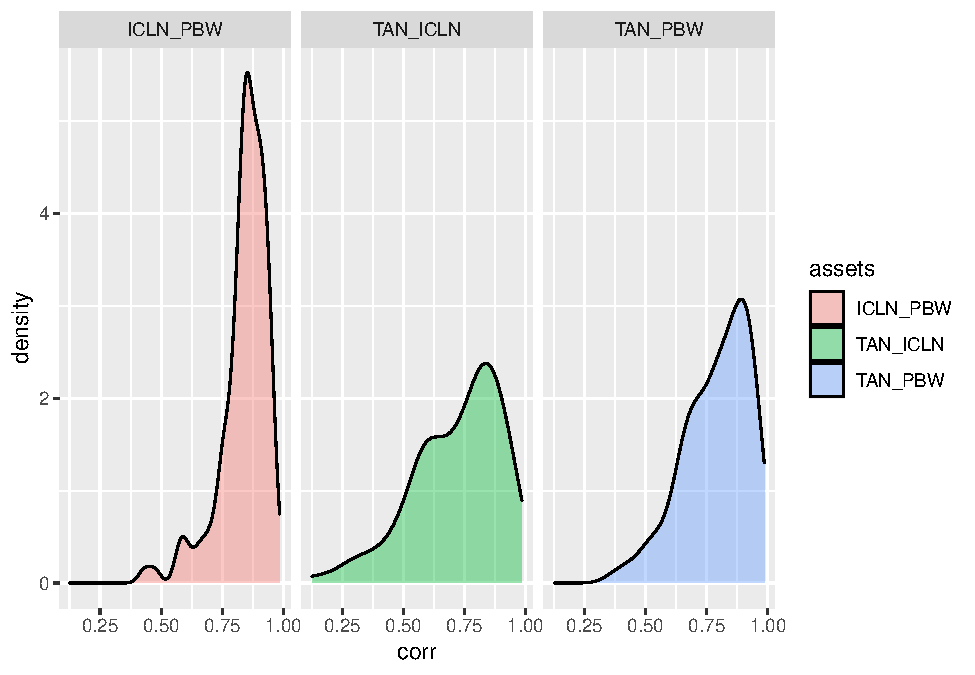
\includegraphics{market-facts_files/figure-latex/explorecorr-1.pdf}

\begin{Shaded}
\begin{Highlighting}[]
\CommentTok{\#}
\NormalTok{corr\_tbl }\SpecialCharTok{\%\textgreater{}\%} \FunctionTok{ggplot}\NormalTok{(}\FunctionTok{aes}\NormalTok{(}\AttributeTok{x =}\NormalTok{ date, }\AttributeTok{y =}\NormalTok{ corr, }\AttributeTok{color =}\NormalTok{ assets)) }\SpecialCharTok{+}
  \FunctionTok{geom\_line}\NormalTok{() }\SpecialCharTok{+} 
  \FunctionTok{facet\_wrap}\NormalTok{(}\SpecialCharTok{\textasciitilde{}}\NormalTok{assets)}
\end{Highlighting}
\end{Shaded}

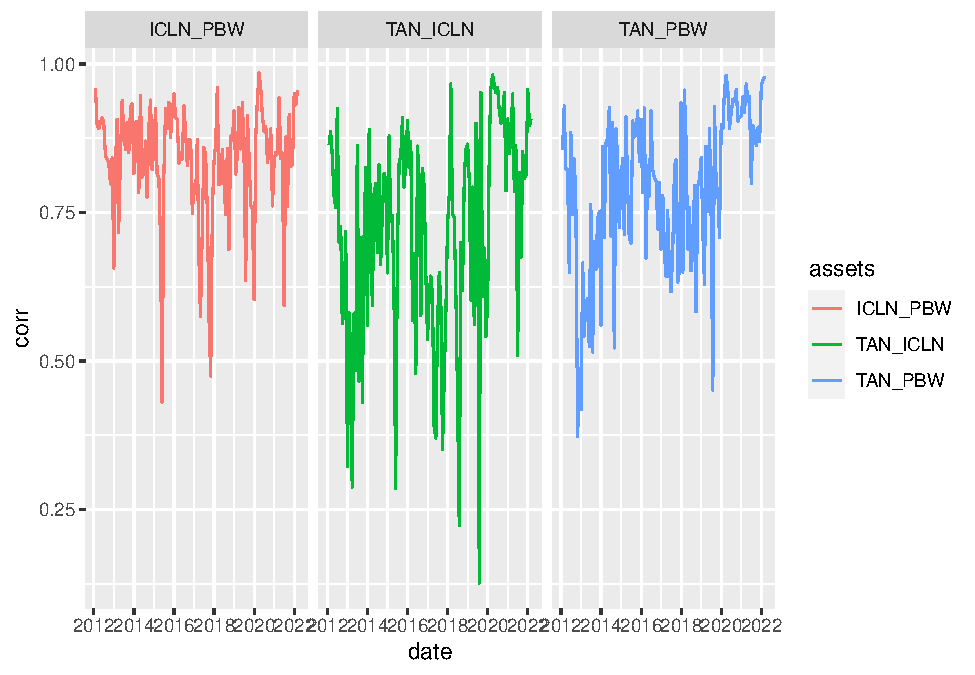
\includegraphics{market-facts_files/figure-latex/explorecorr-2.pdf}

\begin{Shaded}
\begin{Highlighting}[]
\CommentTok{\#}
\end{Highlighting}
\end{Shaded}

These plots not only support the summary statistics, but they also
illustrate the phenomenon of volatility clustering effectively.

We use the right column of \texttt{vols\_tbl}, namely, \texttt{vols}.

\begin{Shaded}
\begin{Highlighting}[]
\CommentTok{\#}
\NormalTok{vols\_tbl }\SpecialCharTok{\%\textgreater{}\%} \FunctionTok{ggplot}\NormalTok{(}\FunctionTok{aes}\NormalTok{(}\AttributeTok{x =}\NormalTok{ vols, }\AttributeTok{fill =}\NormalTok{ assets)) }\SpecialCharTok{+} 
  \FunctionTok{geom\_density}\NormalTok{(}\AttributeTok{alpha =} \FloatTok{0.4}\NormalTok{) }\SpecialCharTok{+} 
  \FunctionTok{facet\_wrap}\NormalTok{(}\SpecialCharTok{\textasciitilde{}}\NormalTok{assets)}
\end{Highlighting}
\end{Shaded}

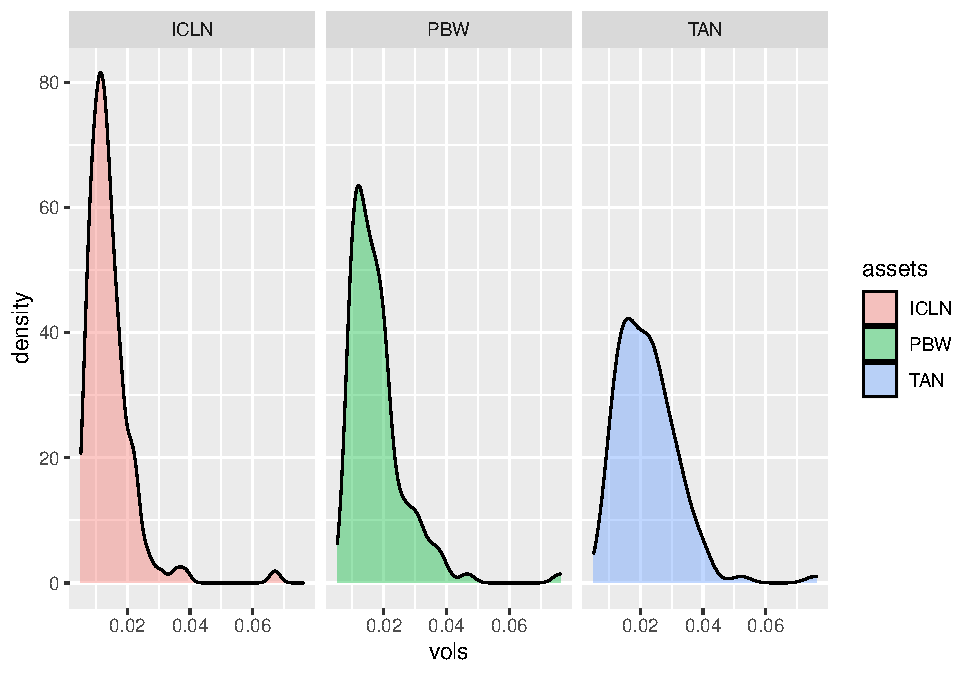
\includegraphics{market-facts_files/figure-latex/vols-ex-1.pdf}

\begin{Shaded}
\begin{Highlighting}[]
\CommentTok{\#}
\NormalTok{vols\_tbl }\SpecialCharTok{\%\textgreater{}\%} \FunctionTok{ggplot}\NormalTok{(}\FunctionTok{aes}\NormalTok{(}\AttributeTok{x =}\NormalTok{ date, }\AttributeTok{y =}\NormalTok{ vols, }\AttributeTok{color =}\NormalTok{ assets)) }\SpecialCharTok{+}
  \FunctionTok{geom\_line}\NormalTok{() }\SpecialCharTok{+} 
  \FunctionTok{facet\_wrap}\NormalTok{(}\SpecialCharTok{\textasciitilde{}}\NormalTok{assets)}
\end{Highlighting}
\end{Shaded}

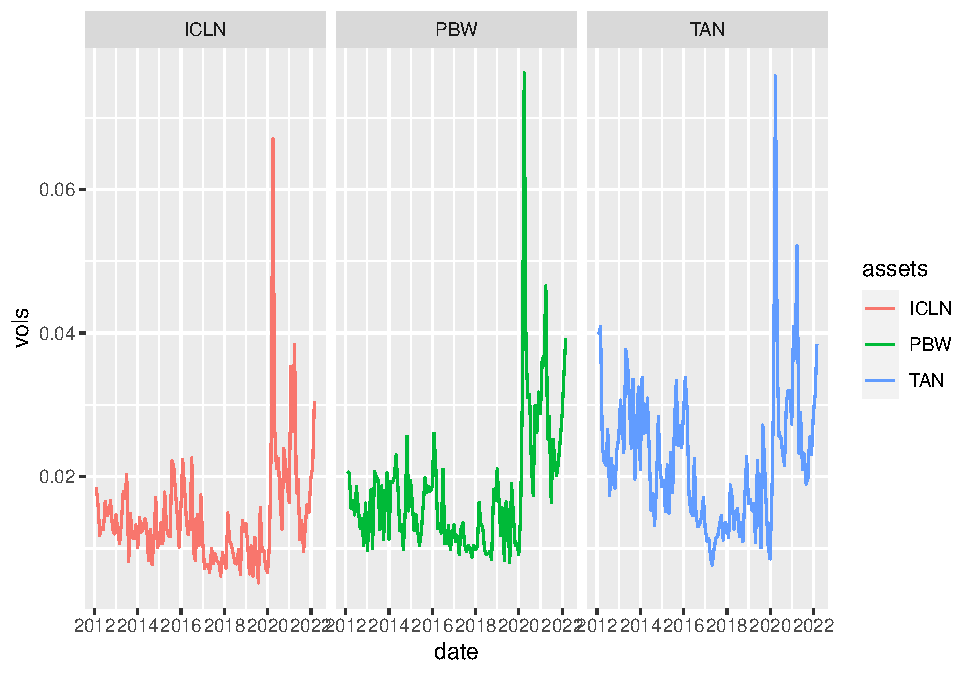
\includegraphics{market-facts_files/figure-latex/vols-ex-2.pdf}

\begin{Shaded}
\begin{Highlighting}[]
\CommentTok{\#}
\end{Highlighting}
\end{Shaded}

These initial forays into exploring the data clearly indicate the highly
volatile nature both of correlation and volatility. The shape of the
data shows prominent right skews and potentially thick tails as well.
All of these point to the existing stylized facts of financial market
returns.

\hypertarget{do-volatility-and-correlation-persist}{%
\subsection{Do volatility and correlation
persist?}\label{do-volatility-and-correlation-persist}}

with the \texttt{TAN\_ICLN} interactions and using the ggplot2 function
\texttt{ggtsdisplay()} from the \texttt{forecast} package, we get all of
this at one stop on the way.

\begin{Shaded}
\begin{Highlighting}[]
\NormalTok{TAN\_ICLN }\OtherTok{\textless{}{-}}\NormalTok{ r\_corr}\SpecialCharTok{$}\NormalTok{TAN\_ICLN}
\NormalTok{forecast}\SpecialCharTok{::}\FunctionTok{ggtsdisplay}\NormalTok{(TAN\_ICLN, }\AttributeTok{lag.max=}\DecValTok{30}\NormalTok{, }\AttributeTok{plot.type =} \StringTok{"histogram"}\NormalTok{)}
\end{Highlighting}
\end{Shaded}

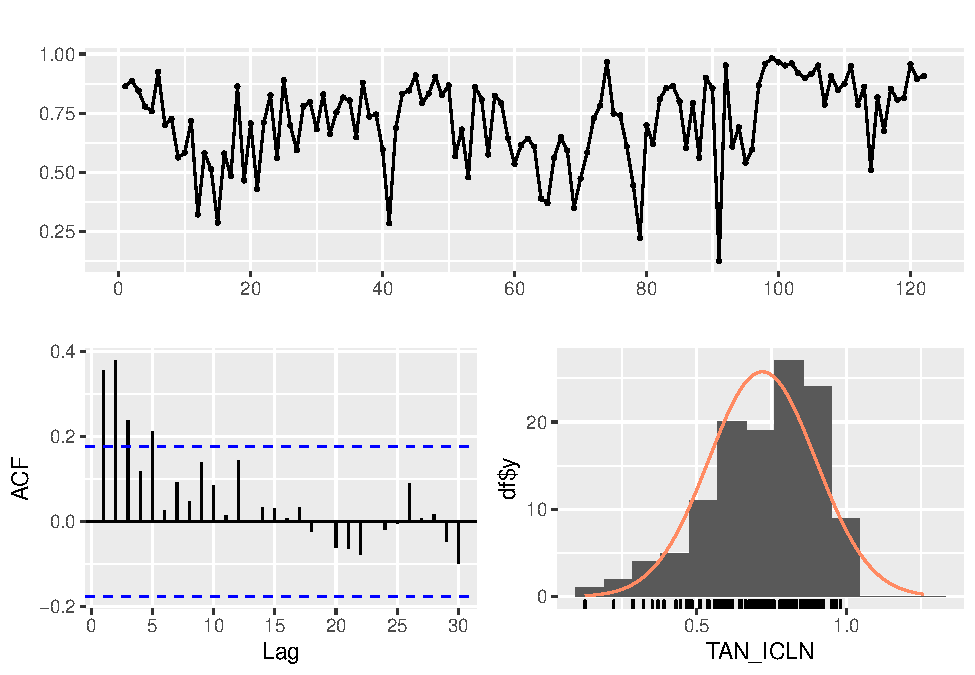
\includegraphics{market-facts_files/figure-latex/persistcorr-1.pdf}

The verdict on correlation persistence?

\begin{itemize}
\item
  There is some monthly persistence to 5 lags.
\item
  The variability of correlation varies only in the positive direction.
\item
  The distribution seems skewed to the left and non-normal.
\end{itemize}

We check the \texttt{TAN} volatilities next.

\begin{Shaded}
\begin{Highlighting}[]
\NormalTok{TAN }\OtherTok{\textless{}{-}}\NormalTok{ r\_vols}\SpecialCharTok{$}\NormalTok{TAN}
\NormalTok{forecast}\SpecialCharTok{::}\FunctionTok{ggtsdisplay}\NormalTok{(TAN,}\AttributeTok{lag.max=}\DecValTok{30}\NormalTok{, }\AttributeTok{plot.type =} \StringTok{"scatter"}\NormalTok{)}
\end{Highlighting}
\end{Shaded}

What is the verdict on volatility persistence?

\begin{itemize}
\item
  Strong and persistent lags over 10 months shows slow decay. Is this
  some evidence of market memory of risk?
\item
  Perhaps, but it also indicates in this monthly time interval
  influences of outliers in the third scatter panel and variability seen
  in the first time series panel.
\end{itemize}

And, perhaps, the term \emph{verdict} is too strong. But we do seem some
recurring patterns in line with previously identified stylizations of
market data.

\hypertarget{do-markets-spill-into-one-another}{%
\section{Do markets spill into one
another?}\label{do-markets-spill-into-one-another}}

Market spillover occurs when the volatility of one market, through
entanglement\footnote{This is a term from quantum mechanics when the
  state of the system (the market here) is indeterminate but nonetheless
  components are correlated. See David Orrell (2020) to peer into these
  ideas.}, affects the volatility of another market. We have three
markets here: TAN, ICLN, and PBW all interacting with one another. We
are not asking why, just the question of whether we observe spillover.
If ICLN is volatile, will TAN be affected? If so, unanticipated
competitive movements in one sector (ICLN) will cause unanticipated
movements in another (TAN), here coupled through correlational
structures, perhaps modeled with copulae.

Let's examine this idea with a simple scatter matrix.

\begin{Shaded}
\begin{Highlighting}[]
\NormalTok{corr\_vols }\OtherTok{\textless{}{-}} \FunctionTok{merge}\NormalTok{(r\_corr, r\_vols)}
\NormalTok{corr\_vols\_tbl }\OtherTok{\textless{}{-}}\NormalTok{ corr\_vols }\SpecialCharTok{\%\textgreater{}\%} \FunctionTok{as\_tibble}\NormalTok{() }\SpecialCharTok{\%\textgreater{}\%} 
  \FunctionTok{mutate}\NormalTok{(}\AttributeTok{date =} \FunctionTok{index}\NormalTok{(corr\_vols)) }
\FunctionTok{ggpairs}\NormalTok{(corr\_vols\_tbl[, }\FunctionTok{c}\NormalTok{(}\StringTok{"TAN\_ICLN"}\NormalTok{, }\StringTok{"ICLN"}\NormalTok{)])}
\end{Highlighting}
\end{Shaded}

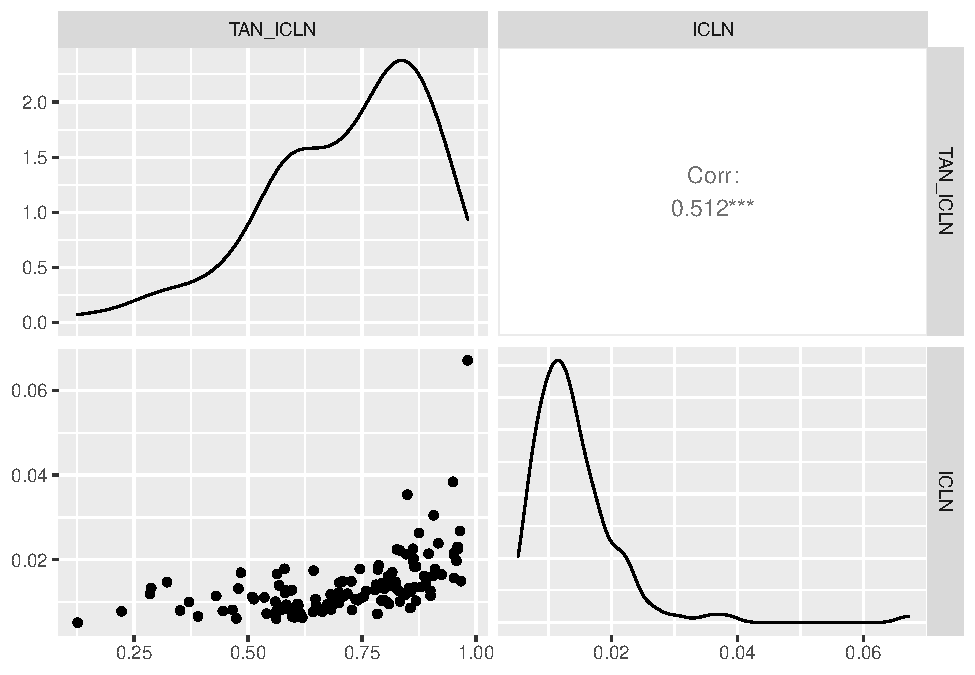
\includegraphics{market-facts_files/figure-latex/pairs-1.pdf}

What do we observe?

\begin{enumerate}
\def\labelenumi{\arabic{enumi}.}
\item
  Are they apparently normally distributed? Not at all, apparently. We
  observe a negative skew in correlation and the characteristically
  positive skew in volatility.
\item
  What do the outliers look like in a potential relationship between
  correlations and volatility? The scatter plot indicates potential
  outliers in very high and very low correlation market environments.
\item
  Are there potentially multiple regions of outliers? Yes, in very high
  and low correlation environments. The body of the relation appears to
  have a positive impact in line with a fairly high correlation of
  0.513.
\end{enumerate}

\hypertarget{quantile-regression-thoughts}{%
\subsection{Quantile regression
thoughts}\label{quantile-regression-thoughts}}

With the existence of outliers in multiple regions we might consider a
technique that respects this situation. That technique is quantile
regression using the \texttt{quantreg} package. Quantile regression
(Koenker (2005)) can help us measure the impact of high stress episodes
on markets, modeled as high and low quantiles.\footnote{Here is a
  \href{https://turing.manhattan.edu/~wfoote01/finalytics/primer-quantile-regression.html}{tutorial
  on quantile regression} that is helpful for the formulation of models
  and the interpretation of results.}

\begin{itemize}
\item
  Just like \texttt{lm()}for Ordinary Leasat Squares (OLS), we set up
  \texttt{rq()} with left-hand side (correlations) and right hand side
  variables (volatilities).
\item
  We also specify the quantiles of the left-hand side to identify
  outliers and the median of the relationship using the \texttt{taus}
  vector. Each value of \texttt{tau} will run a separate regression.
\end{itemize}

We run this code for one combination of correlations and volatilities.
We can modify \texttt{y} and \texttt{x} for other combinations, and
thus, other markets. A log-log transformation can help us understand the
relationship between markets as the elasticity of correlation with
respect to volatility.

\begin{Shaded}
\begin{Highlighting}[]
\FunctionTok{library}\NormalTok{(quantreg)}
\NormalTok{taus }\OtherTok{\textless{}{-}} \FunctionTok{c}\NormalTok{(}\FloatTok{0.10}\NormalTok{, }\FloatTok{0.25}\NormalTok{, }\FloatTok{0.50}\NormalTok{, }\FloatTok{0.75}\NormalTok{, }\FloatTok{0.90}\NormalTok{) }\CommentTok{\# quantiles of y for a 95\% confidence interval}
\NormalTok{y }\OtherTok{\textless{}{-}}\NormalTok{ corr\_vols\_tbl}\SpecialCharTok{$}\NormalTok{TAN\_ICLN; x }\OtherTok{\textless{}{-}}\NormalTok{ corr\_vols\_tbl}\SpecialCharTok{$}\NormalTok{ICLN}
\NormalTok{fit\_corr\_vols }\OtherTok{\textless{}{-}} \FunctionTok{rq}\NormalTok{(}\FunctionTok{log}\NormalTok{(y) }\SpecialCharTok{\textasciitilde{}} \FunctionTok{log}\NormalTok{(x), }\AttributeTok{tau =}\NormalTok{ taus)}
\NormalTok{fit\_summary }\OtherTok{\textless{}{-}} \FunctionTok{summary}\NormalTok{(fit\_corr\_vols)}
\NormalTok{fit\_summary}
\end{Highlighting}
\end{Shaded}

\begin{verbatim}
## 
## Call: rq(formula = log(y) ~ log(x), tau = taus)
## 
## tau: [1] 0.1
## 
## Coefficients:
##             coefficients lower bd upper bd
## (Intercept) 1.0691       1.0581   2.0181  
## log(x)      0.4011       0.3663   0.6394  
## 
## Call: rq(formula = log(y) ~ log(x), tau = taus)
## 
## tau: [1] 0.25
## 
## Coefficients:
##             coefficients lower bd upper bd
## (Intercept) 1.2070       0.7607   1.7363  
## log(x)      0.3739       0.2745   0.5402  
## 
## Call: rq(formula = log(y) ~ log(x), tau = taus)
## 
## tau: [1] 0.5
## 
## Coefficients:
##             coefficients lower bd upper bd
## (Intercept) 1.1664       0.8762   1.3282  
## log(x)      0.3356       0.2677   0.3776  
## 
## Call: rq(formula = log(y) ~ log(x), tau = taus)
## 
## tau: [1] 0.75
## 
## Coefficients:
##             coefficients lower bd upper bd
## (Intercept) 1.0588       0.5676   1.5113  
## log(x)      0.2893       0.1730   0.4017  
## 
## Call: rq(formula = log(y) ~ log(x), tau = taus)
## 
## tau: [1] 0.9
## 
## Coefficients:
##             coefficients lower bd upper bd
## (Intercept) 0.6690       0.5599   1.6484  
## log(x)      0.1857       0.1313   0.3975
\end{verbatim}

\begin{Shaded}
\begin{Highlighting}[]
\FunctionTok{plot}\NormalTok{(fit\_summary)}
\end{Highlighting}
\end{Shaded}

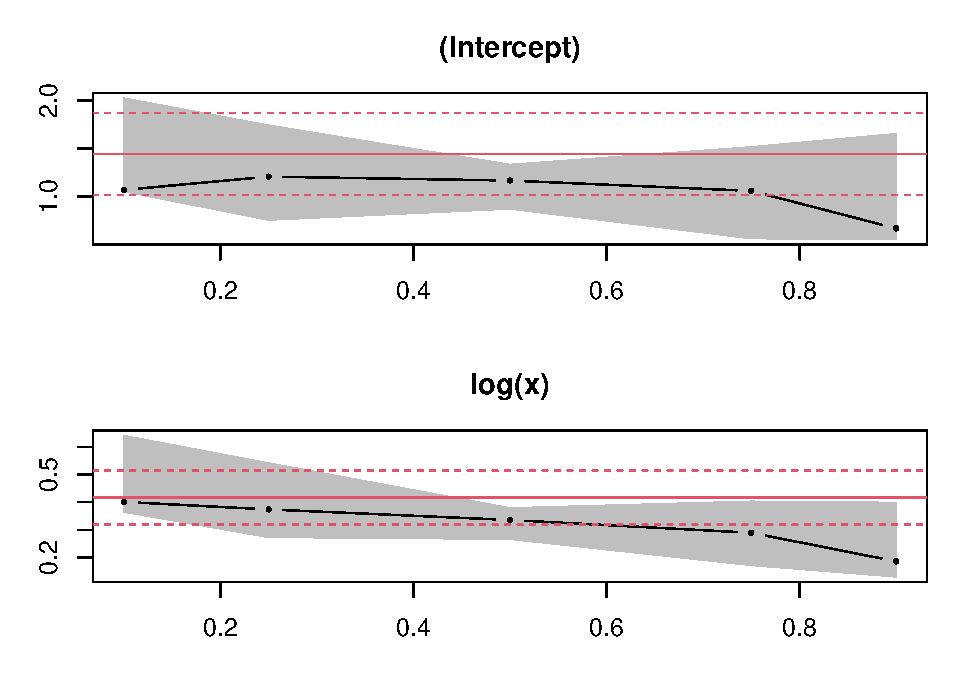
\includegraphics{market-facts_files/figure-latex/quantile-1.pdf}

The plot depicts the parameter estimate (intercept and slope) on the
vertical axis and the quantile of correlation on the horizontal axis.
The gray range is the 95\% confidence interval of the parameter
estimates. The dashed red lines depict the ordinary least squares
regression confidence intervals.

We might ask further questions of this analysis.

\begin{enumerate}
\def\labelenumi{\arabic{enumi}.}
\item
  When is it likely for markets to spill over? Mostly across low to high
  correlation quantiles.
\item
  At what likelihood of correlations are market spillovers most
  uncertain? Again in very low and very high correlation quantile
  regions.
\item
  What about the other markets and their spillover effects?
\item
  What should the CFO glean from from these results?
\end{enumerate}

The last two questions deserve further analysis, which means more
regressions. The CFO can get an idea that preparing for market risk is a
very high risk management priority.

One more plot to tie up the market spillover questions.

\begin{Shaded}
\begin{Highlighting}[]
\NormalTok{p }\OtherTok{\textless{}{-}} \FunctionTok{ggplot}\NormalTok{(corr\_vols\_tbl,  }\FunctionTok{aes}\NormalTok{(}\AttributeTok{x =}\NormalTok{ ICLN, }\AttributeTok{y =}\NormalTok{ TAN\_ICLN)) }\SpecialCharTok{+}
    \FunctionTok{geom\_point}\NormalTok{() }\SpecialCharTok{+} 
    \FunctionTok{ggtitle}\NormalTok{(}\StringTok{"TAN{-}ICLN Interaction"}\NormalTok{) }\SpecialCharTok{+} 
    \FunctionTok{geom\_quantile}\NormalTok{(}\AttributeTok{quantiles =} \FunctionTok{c}\NormalTok{(}\FloatTok{0.10}\NormalTok{, }\FloatTok{0.90}\NormalTok{)) }\SpecialCharTok{+} 
    \FunctionTok{geom\_quantile}\NormalTok{(}\AttributeTok{quantiles =} \FloatTok{0.5}\NormalTok{, }\AttributeTok{linetype =} \StringTok{"longdash"}\NormalTok{) }\SpecialCharTok{+}
    \FunctionTok{geom\_density\_2d}\NormalTok{(}\AttributeTok{colour =} \StringTok{"red"}\NormalTok{)  }
\NormalTok{p}
\end{Highlighting}
\end{Shaded}

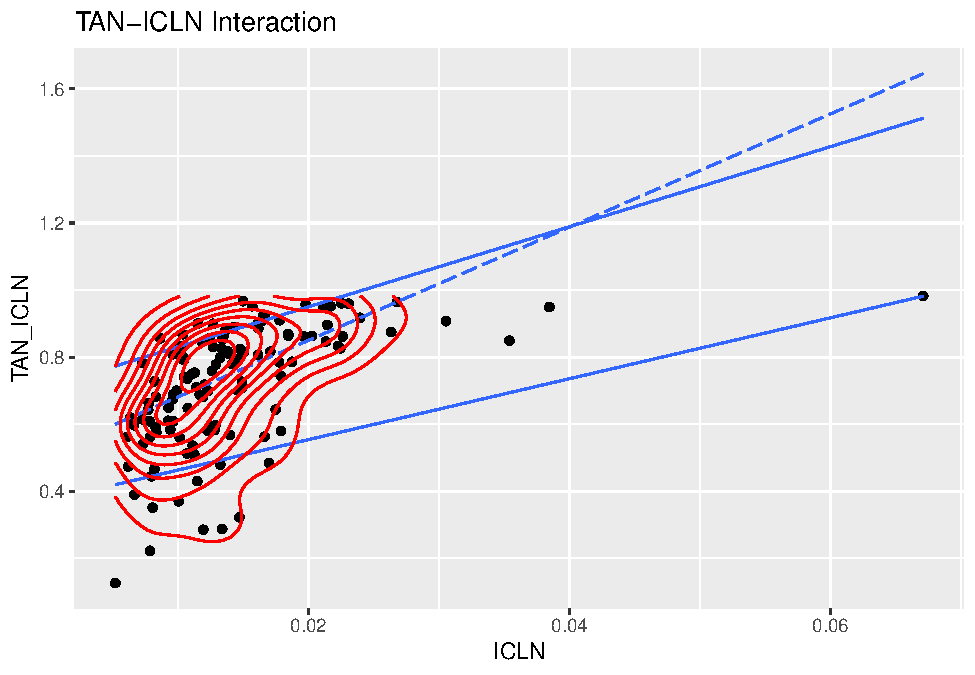
\includegraphics{market-facts_files/figure-latex/rqplot-1.pdf}

To tailor this picture a bit, we can use \texttt{+\ ylim(0.25,\ 1)} to
specify the y-axis limits. The dashed line depicts the 50th quantile.

To what degree do our conclusions change when we perform similar
analyses on the other market interactions? {[}TO BE DETERMINED{]}

\hypertarget{bayesian-thoughts}{%
\subsection{Bayesian thoughts}\label{bayesian-thoughts}}

Alternatively, we can examine the impact of the riskiness of one market
on the other using a probabilistic model. Up to this point we have
implemented a robust, perhaps in a frequentist mood, model of market
interaction. This allows us to form a binary hypothesis: \(H_0\) no
spillover, and \(H_1\) spillover. We might question the acceptance or
rejection of hypotheses based on the probably emphasis on the null
hypothesis. We might also observe overlap of the probability that either
might occur.

This objection raises the issue of prior expectations about the
hypotheses. If we assume that each is equally probable, perhaps \(Beta\)
distributed then we could let the likelihood of each hypothesis directly
impact our inference. If we were to update priors with posteriors, we
might also be able to tune the inference further.

Inherently these are not complex models with only a single regressor
acting on a dependent variable. Built into each variate are several
assumptions about the variability and co-variability of returns. We
might ask next what is the industry structure of spillover effects, at
least as represented by these three segments of the renewables market.

We propose this generative model.

\begin{align}
\rho_[i] & \sim \operatorname{Normal}(\mu_{\rho}, \sigma_{\rho}) \\
\mu_{\rho [i]} &= \alpha_[i] + \beta_[i] \sigma_[i] \\
\alpha_[i] & \sim \operatorname{Normal}(0,1) \\
\beta_[i] & \sim \operatorname{Normal}(0,1) \\
\sigma_{\rho [i]} & \sim \operatorname{Exp}(1) \\
\end{align}

The markets are indicated by \([i]\), with \(\rho\) and \(\sigma\) the
within-month correlation and market volatility, \(\mu_{\rho}\) and
\(\sigma_{\rho}\) the expected value and volatility of the relationship
between within-month correlation and market volatility. This formulation
allows a mixed-random effects hierarchical model of the probably market
risk infrastructure.

\begin{Shaded}
\begin{Highlighting}[]
\FunctionTok{library}\NormalTok{(rethinking)}
\NormalTok{y }\OtherTok{\textless{}{-}}\NormalTok{ corr\_vols\_tbl}\SpecialCharTok{$}\NormalTok{TAN\_ICLN; x }\OtherTok{\textless{}{-}}\NormalTok{ corr\_vols\_tbl}\SpecialCharTok{$}\NormalTok{ICLN}
\NormalTok{d\_1 }\OtherTok{\textless{}{-}} \FunctionTok{tibble}\NormalTok{(}
  \AttributeTok{tan\_icln =}\NormalTok{ y,}
  \AttributeTok{icln =}\NormalTok{ x}
\NormalTok{)}
\NormalTok{m\_1 }\OtherTok{\textless{}{-}} \FunctionTok{quap}\NormalTok{(}
  \FunctionTok{alist}\NormalTok{(}
\NormalTok{    tan\_icln }\SpecialCharTok{\textasciitilde{}} \FunctionTok{dnorm}\NormalTok{( mu, sigma ),}
\NormalTok{    mu }\OtherTok{\textless{}{-}}\NormalTok{ a }\SpecialCharTok{+}\NormalTok{ b}\SpecialCharTok{*}\NormalTok{icln,}
\NormalTok{    a }\SpecialCharTok{\textasciitilde{}} \FunctionTok{dnorm}\NormalTok{( }\DecValTok{0}\NormalTok{, }\DecValTok{1}\NormalTok{ ),}
\NormalTok{    b }\SpecialCharTok{\textasciitilde{}} \FunctionTok{dnorm}\NormalTok{( }\DecValTok{0}\NormalTok{, }\DecValTok{1}\NormalTok{ ),}
\NormalTok{    sigma }\SpecialCharTok{\textasciitilde{}} \FunctionTok{dexp}\NormalTok{( }\DecValTok{1}\NormalTok{ )}
\NormalTok{  ),}
  \AttributeTok{data =}\NormalTok{ d\_1}
\NormalTok{)}
\FunctionTok{precis}\NormalTok{( m\_1 )}
\end{Highlighting}
\end{Shaded}

\begin{verbatim}
##         mean      sd   5.5%  94.5%
## a     0.6857 0.02035 0.6532 0.7182
## b     2.3440 0.93356 0.8520 3.8360
## sigma 0.1706 0.01132 0.1525 0.1887
\end{verbatim}

Priors are proper to the generation of the dependent variable. They can
also take on positive or negative signs. Spillover is much in evidence
here through size of impact and direction. Let's repeat this for the
TAN-PBW and PBW-ICLN markets separately.

\begin{Shaded}
\begin{Highlighting}[]
\CommentTok{\#library(rethinking)}
\NormalTok{y }\OtherTok{\textless{}{-}}\NormalTok{ corr\_vols\_tbl}\SpecialCharTok{$}\NormalTok{TAN\_PBW; x }\OtherTok{\textless{}{-}}\NormalTok{ corr\_vols\_tbl}\SpecialCharTok{$}\NormalTok{PBW}
\NormalTok{d\_2 }\OtherTok{\textless{}{-}} \FunctionTok{tibble}\NormalTok{(}
  \AttributeTok{tan\_pbw =}\NormalTok{ y,}
  \AttributeTok{pbw =}\NormalTok{ x}
\NormalTok{)}
\NormalTok{m\_2 }\OtherTok{\textless{}{-}} \FunctionTok{quap}\NormalTok{(}
  \FunctionTok{alist}\NormalTok{(}
\NormalTok{    tan\_pbw }\SpecialCharTok{\textasciitilde{}} \FunctionTok{dnorm}\NormalTok{( mu, sigma ),}
\NormalTok{    mu }\OtherTok{\textless{}{-}}\NormalTok{ a }\SpecialCharTok{+}\NormalTok{ b}\SpecialCharTok{*}\NormalTok{pbw,}
\NormalTok{    a }\SpecialCharTok{\textasciitilde{}} \FunctionTok{dnorm}\NormalTok{( }\DecValTok{0}\NormalTok{, }\DecValTok{1}\NormalTok{ ),}
\NormalTok{    b }\SpecialCharTok{\textasciitilde{}} \FunctionTok{dnorm}\NormalTok{( }\DecValTok{0}\NormalTok{, }\DecValTok{1}\NormalTok{ ),}
\NormalTok{    sigma }\SpecialCharTok{\textasciitilde{}} \FunctionTok{dexp}\NormalTok{( }\DecValTok{1}\NormalTok{ )}
\NormalTok{  ),}
  \AttributeTok{data =}\NormalTok{ d\_2}
\NormalTok{)}
\FunctionTok{precis}\NormalTok{( m\_2 )}
\end{Highlighting}
\end{Shaded}

\begin{verbatim}
##         mean       sd   5.5%  94.5%
## a     0.7285 0.017928 0.6998 0.7571
## b     3.4235 0.804827 2.1372 4.7097
## sigma 0.1186 0.008041 0.1058 0.1315
\end{verbatim}

A comparatively stronger influence is felt in this market interaction.
Now for the last pair, ICLN\_PBW.

\begin{Shaded}
\begin{Highlighting}[]
\CommentTok{\#library(rethinking)}
\NormalTok{y }\OtherTok{\textless{}{-}}\NormalTok{ corr\_vols\_tbl}\SpecialCharTok{$}\NormalTok{ICLN\_PBW; x }\OtherTok{\textless{}{-}}\NormalTok{ corr\_vols\_tbl}\SpecialCharTok{$}\NormalTok{PBW}
\NormalTok{d\_3 }\OtherTok{\textless{}{-}} \FunctionTok{tibble}\NormalTok{(}
  \AttributeTok{icln\_pbw =}\NormalTok{ y,}
  \AttributeTok{pbw =}\NormalTok{ x}
\NormalTok{)}
\NormalTok{m\_3 }\OtherTok{\textless{}{-}} \FunctionTok{quap}\NormalTok{(}
  \FunctionTok{alist}\NormalTok{(}
\NormalTok{    icln\_pbw }\SpecialCharTok{\textasciitilde{}} \FunctionTok{dnorm}\NormalTok{( mu, sigma ),}
\NormalTok{    mu }\OtherTok{\textless{}{-}}\NormalTok{ a }\SpecialCharTok{+}\NormalTok{ b}\SpecialCharTok{*}\NormalTok{pbw,}
\NormalTok{    a }\SpecialCharTok{\textasciitilde{}} \FunctionTok{dnorm}\NormalTok{( }\DecValTok{0}\NormalTok{, }\DecValTok{1}\NormalTok{ ),}
\NormalTok{    b }\SpecialCharTok{\textasciitilde{}} \FunctionTok{dnorm}\NormalTok{( }\DecValTok{0}\NormalTok{, }\DecValTok{1}\NormalTok{ ),}
\NormalTok{    sigma }\SpecialCharTok{\textasciitilde{}} \FunctionTok{dexp}\NormalTok{( }\DecValTok{1}\NormalTok{ )}
\NormalTok{  ),}
  \AttributeTok{data =}\NormalTok{ d\_3}
\NormalTok{)}
\FunctionTok{precis}\NormalTok{( m\_3 )}
\end{Highlighting}
\end{Shaded}

\begin{verbatim}
##          mean       sd    5.5%   94.5%
## a     0.78979 0.014424 0.76674 0.81284
## b     2.77513 0.673484 1.69877 3.85149
## sigma 0.08815 0.005795 0.07889 0.09741
\end{verbatim}

Wind and solar seem to have similar spilloever characteristics relative
to clean technologies. All of the models have similarities to the
quantile regressions.

Pareto-Smoothed Importance Sampling and cross validation with the Leave
One Out approach gives us the trade-off between spillover variability
and bias on the y-axis and uncertainty on the x-axis. Thick-tailed,
skewed returns distributions get their intelligibility with this
analysis. The extreme uncertainty of the outliers (known-unknowns from
\(k\) = 0 to 0.7; unknown-unknowns for \(k\) \textgreater{} 0.7 in tests
reported by Gelman and Vehtari (2013) and Vehtari and Gabry (2015) )
contributes to the ability of the ICLN market to spill its uncertainty
into the high variations of the TAN market all through the naive
mechanism of correlation.\footnote{Power law distributions notoriously
  do not possess first, second, third, or even fourth moments
  analytically across the GPD parameter space, especially for \(k\) (see
  Embrechts (2000) for examples). This divergent feature means we should
  rely on the more robust median, mean absolute deviation, and
  inter-quartile ranges (probability intervals) to summarize the
  outcomes of power law distributions.}

\begin{Shaded}
\begin{Highlighting}[]
\DocumentationTok{\#\# R code 7.34 McElreath2020}
\CommentTok{\#library( plotly )}
\FunctionTok{options}\NormalTok{( }\AttributeTok{digits=}\DecValTok{2}\NormalTok{, }\AttributeTok{scipen=}\DecValTok{999999}\NormalTok{)}
\NormalTok{d }\OtherTok{\textless{}{-}}\NormalTok{ d\_1}
\FunctionTok{set.seed}\NormalTok{(}\DecValTok{4284}\NormalTok{)}
\NormalTok{m }\OtherTok{\textless{}{-}}\NormalTok{ m\_1}
\NormalTok{PSIS\_m }\OtherTok{\textless{}{-}} \FunctionTok{PSIS}\NormalTok{( m, }\AttributeTok{pointwise=}\ConstantTok{TRUE}\NormalTok{ )}
\NormalTok{PSIS\_m }\OtherTok{\textless{}{-}} \FunctionTok{cbind}\NormalTok{( PSIS\_m, }\AttributeTok{tan\_icln=}\NormalTok{d}\SpecialCharTok{$}\NormalTok{tan\_icln, }\AttributeTok{icln=}\NormalTok{d}\SpecialCharTok{$}\NormalTok{icln )}
\FunctionTok{set.seed}\NormalTok{(}\DecValTok{4284}\NormalTok{)}
\CommentTok{\#WAIC\_m2.2 \textless{}{-} WAIC(m2.2,pointwise=TRUE)}
\NormalTok{p1 }\OtherTok{\textless{}{-}}\NormalTok{ PSIS\_m }\SpecialCharTok{\%\textgreater{}\%} 
  \FunctionTok{ggplot}\NormalTok{( }\FunctionTok{aes}\NormalTok{( }\AttributeTok{x=}\NormalTok{penalty, }\AttributeTok{y=}\NormalTok{k ) ) }\SpecialCharTok{+}
  \FunctionTok{geom\_point}\NormalTok{( }\AttributeTok{shape=}\DecValTok{21}\NormalTok{, }\AttributeTok{color =} \StringTok{"blue"}\NormalTok{ ) }\SpecialCharTok{+} 
  \FunctionTok{xlab}\NormalTok{(}\StringTok{"PSIS Pareto k"}\NormalTok{) }\SpecialCharTok{+} \FunctionTok{ylab}\NormalTok{(}\StringTok{"PSIS penalty"}\NormalTok{) }\SpecialCharTok{+} 
  \FunctionTok{geom\_vline}\NormalTok{( }\AttributeTok{xintercept =} \FloatTok{0.7}\NormalTok{, }\AttributeTok{linetype =} \StringTok{"dashed"}\NormalTok{) }\SpecialCharTok{+} 
  \FunctionTok{ggtitle}\NormalTok{( }\StringTok{"ICLN spills over into TAN"}\NormalTok{ )}
\NormalTok{p1 }\CommentTok{\#ggplotly( p1 )}
\end{Highlighting}
\end{Shaded}

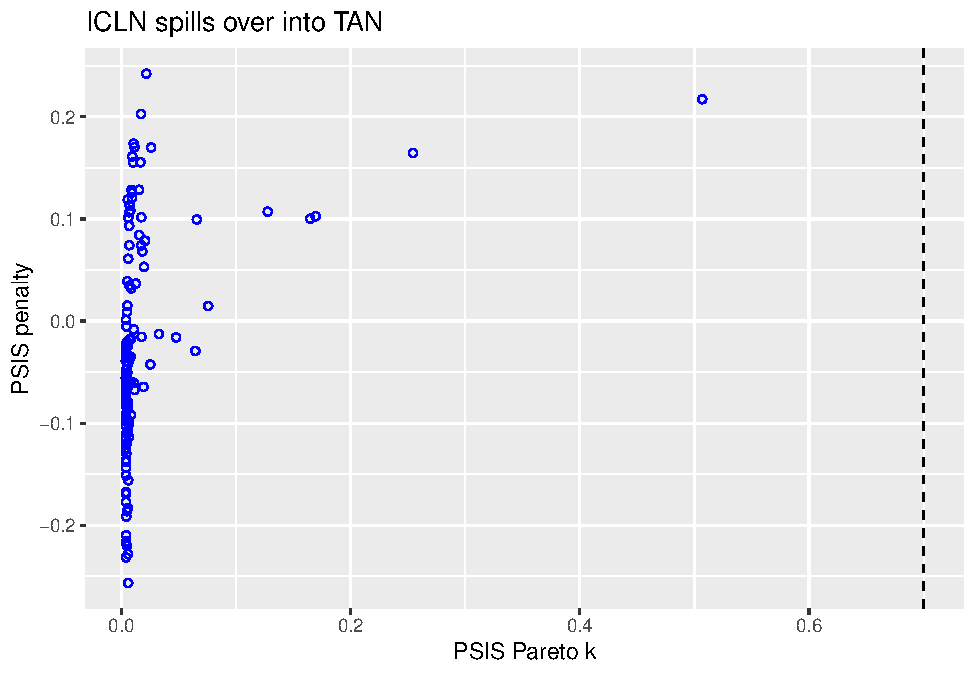
\includegraphics{market-facts_files/figure-latex/psis-k-penalty-1.pdf}

Here are the TAN-PBW outlier results.

\begin{Shaded}
\begin{Highlighting}[]
\DocumentationTok{\#\# R code 7.34 McElreath2020}
\FunctionTok{library}\NormalTok{( plotly )}
\FunctionTok{options}\NormalTok{( }\AttributeTok{digits=}\DecValTok{2}\NormalTok{, }\AttributeTok{scipen=}\DecValTok{999999}\NormalTok{)}
\NormalTok{d }\OtherTok{\textless{}{-}}\NormalTok{ d\_2}
\FunctionTok{set.seed}\NormalTok{(}\DecValTok{4284}\NormalTok{)}
\NormalTok{m }\OtherTok{\textless{}{-}}\NormalTok{ m\_2}
\NormalTok{PSIS\_m }\OtherTok{\textless{}{-}} \FunctionTok{PSIS}\NormalTok{( m, }\AttributeTok{pointwise=}\ConstantTok{TRUE}\NormalTok{ )}
\NormalTok{PSIS\_m }\OtherTok{\textless{}{-}} \FunctionTok{cbind}\NormalTok{( PSIS\_m, }\AttributeTok{tan\_pbw=}\NormalTok{d}\SpecialCharTok{$}\NormalTok{tan\_pbw, }\AttributeTok{icln=}\NormalTok{d}\SpecialCharTok{$}\NormalTok{pbw )}
\FunctionTok{set.seed}\NormalTok{(}\DecValTok{4284}\NormalTok{)}
\CommentTok{\#WAIC\_m2.2 \textless{}{-} WAIC(m2.2,pointwise=TRUE)}
\NormalTok{p1 }\OtherTok{\textless{}{-}}\NormalTok{ PSIS\_m }\SpecialCharTok{\%\textgreater{}\%} 
  \FunctionTok{ggplot}\NormalTok{( }\FunctionTok{aes}\NormalTok{( }\AttributeTok{x=}\NormalTok{penalty, }\AttributeTok{y=}\NormalTok{k ) ) }\SpecialCharTok{+}
  \FunctionTok{geom\_point}\NormalTok{( }\AttributeTok{shape=}\DecValTok{21}\NormalTok{, }\AttributeTok{color =} \StringTok{"blue"}\NormalTok{ ) }\SpecialCharTok{+} 
  \FunctionTok{xlab}\NormalTok{(}\StringTok{"PSIS Pareto k"}\NormalTok{) }\SpecialCharTok{+} \FunctionTok{ylab}\NormalTok{(}\StringTok{"PSIS penalty"}\NormalTok{) }\SpecialCharTok{+} 
  \FunctionTok{geom\_vline}\NormalTok{( }\AttributeTok{xintercept =} \FloatTok{0.7}\NormalTok{, }\AttributeTok{linetype =} \StringTok{"dashed"}\NormalTok{) }\SpecialCharTok{+} 
  \FunctionTok{ggtitle}\NormalTok{( }\StringTok{"PBW spills over into TAN"}\NormalTok{ )}
\NormalTok{p1 }\CommentTok{\#ggplotly( p1 )}
\end{Highlighting}
\end{Shaded}

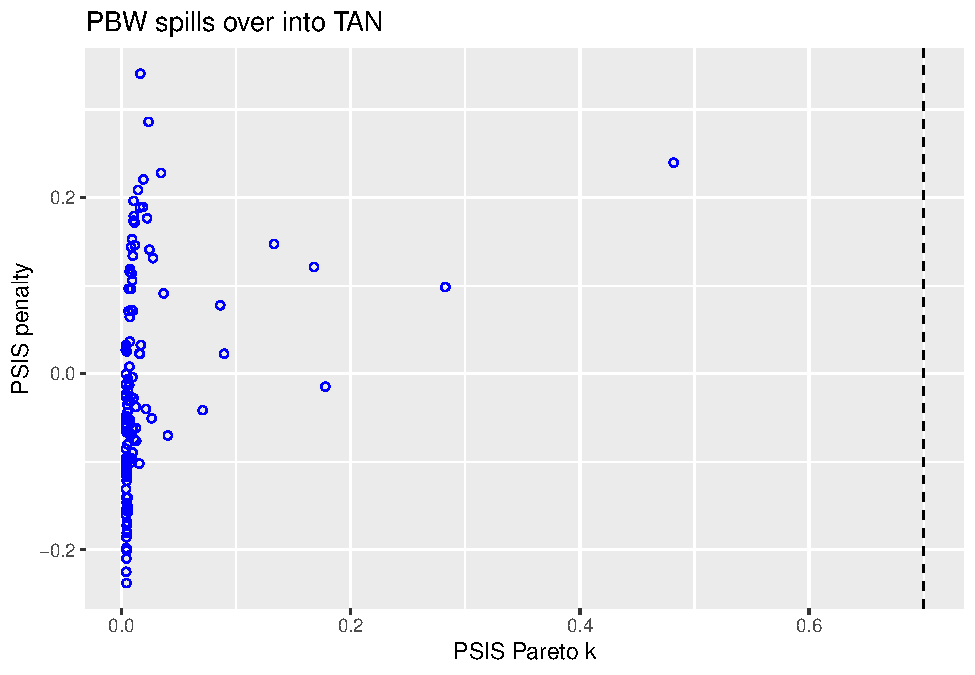
\includegraphics{market-facts_files/figure-latex/psis-spill-tan-pbw-1.pdf}

and

\begin{Shaded}
\begin{Highlighting}[]
\DocumentationTok{\#\# R code 7.34 McElreath2020}
\CommentTok{\#library( plotly )}
\FunctionTok{options}\NormalTok{( }\AttributeTok{digits=}\DecValTok{2}\NormalTok{, }\AttributeTok{scipen=}\DecValTok{999999}\NormalTok{)}
\NormalTok{d }\OtherTok{\textless{}{-}}\NormalTok{ d\_3}
\FunctionTok{set.seed}\NormalTok{(}\DecValTok{4284}\NormalTok{)}
\NormalTok{m }\OtherTok{\textless{}{-}}\NormalTok{ m\_3}
\NormalTok{PSIS\_m }\OtherTok{\textless{}{-}} \FunctionTok{PSIS}\NormalTok{( m, }\AttributeTok{pointwise=}\ConstantTok{TRUE}\NormalTok{ )}
\NormalTok{PSIS\_m }\OtherTok{\textless{}{-}} \FunctionTok{cbind}\NormalTok{( PSIS\_m, }\AttributeTok{icln\_pbw=}\NormalTok{d}\SpecialCharTok{$}\NormalTok{icln\_pbw, }\AttributeTok{pbw=}\NormalTok{d}\SpecialCharTok{$}\NormalTok{pbw )}
\FunctionTok{set.seed}\NormalTok{(}\DecValTok{4284}\NormalTok{)}
\CommentTok{\#WAIC\_m2.2 \textless{}{-} WAIC(m2.2,pointwise=TRUE)}
\NormalTok{p1 }\OtherTok{\textless{}{-}}\NormalTok{ PSIS\_m }\SpecialCharTok{\%\textgreater{}\%} 
  \FunctionTok{ggplot}\NormalTok{( }\FunctionTok{aes}\NormalTok{( }\AttributeTok{x=}\NormalTok{penalty, }\AttributeTok{y=}\NormalTok{k ) ) }\SpecialCharTok{+}
  \FunctionTok{geom\_point}\NormalTok{( }\AttributeTok{shape=}\DecValTok{21}\NormalTok{, }\AttributeTok{color =} \StringTok{"blue"}\NormalTok{ ) }\SpecialCharTok{+} 
  \FunctionTok{xlab}\NormalTok{(}\StringTok{"PSIS Pareto k"}\NormalTok{) }\SpecialCharTok{+} \FunctionTok{ylab}\NormalTok{(}\StringTok{"PSIS penalty"}\NormalTok{) }\SpecialCharTok{+} 
  \FunctionTok{geom\_vline}\NormalTok{( }\AttributeTok{xintercept =} \FloatTok{0.7}\NormalTok{, }\AttributeTok{linetype =} \StringTok{"dashed"}\NormalTok{) }\SpecialCharTok{+} 
  \FunctionTok{ggtitle}\NormalTok{( }\StringTok{"ICLN spills over into PBW"}\NormalTok{ )}
\NormalTok{p1 }\CommentTok{\#ggplotly( p1 )}
\end{Highlighting}
\end{Shaded}

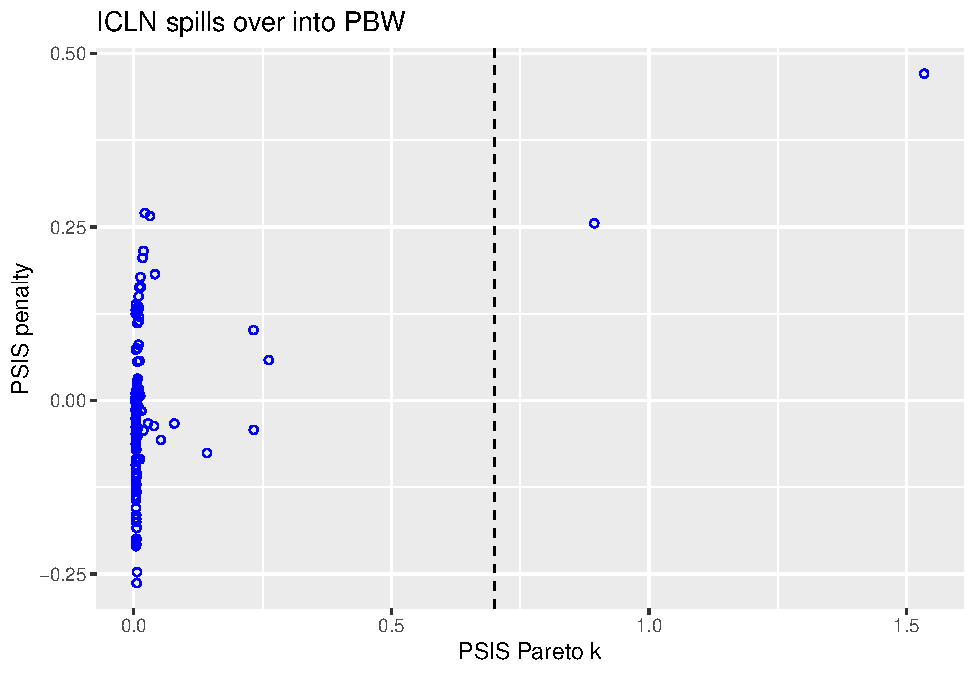
\includegraphics{market-facts_files/figure-latex/psis-spill-pbw-icln-0-1.pdf}

Our next stop is to look at the joint probability of spillover effects
across the three markets.

\hypertarget{industry-risk-infrastructure}{%
\section{Industry risk
infrastructure}\label{industry-risk-infrastructure}}

We now invoke the full generative model, including the jointly
considered markets. We index each market and consider all of the impact
parameters as jointly determined. They thus share information across
markets through the total probability of observing all three markets in
the presence of all of the market interaction parameters.

\begin{Shaded}
\begin{Highlighting}[]
\CommentTok{\#library(rethinking)}
\NormalTok{corr\_vol\_spill }\OtherTok{\textless{}{-}} \FunctionTok{read\_csv}\NormalTok{( }\StringTok{"market{-}spillovers.csv"}\NormalTok{ )}
\NormalTok{d\_4 }\OtherTok{\textless{}{-}}\NormalTok{ corr\_vol\_spill }\SpecialCharTok{\%\textgreater{}\%} 
  \FunctionTok{tibble}\NormalTok{(}
    \AttributeTok{corr =} \FunctionTok{log}\NormalTok{( }\FunctionTok{abs}\NormalTok{(corrs) ),}
    \AttributeTok{vol =} \FunctionTok{log}\NormalTok{( vols ),}
    \AttributeTok{mid =}\NormalTok{ mids}
\NormalTok{)}
\CommentTok{\#log vols and (abs) corrs will allow us to interpret coefficients as elasticities}
\end{Highlighting}
\end{Shaded}

\begin{Shaded}
\begin{Highlighting}[]
\NormalTok{m\_4 }\OtherTok{\textless{}{-}} \FunctionTok{quap}\NormalTok{(}
  \FunctionTok{alist}\NormalTok{(}
\NormalTok{    corr }\SpecialCharTok{\textasciitilde{}} \FunctionTok{dnorm}\NormalTok{( mu, sigma ),}
\NormalTok{    mu }\OtherTok{\textless{}{-}}\NormalTok{ a[mid] }\SpecialCharTok{+}\NormalTok{ b[mid] }\SpecialCharTok{*}\NormalTok{vol,}
\NormalTok{    a[mid] }\SpecialCharTok{\textasciitilde{}} \FunctionTok{dnorm}\NormalTok{( }\DecValTok{0}\NormalTok{, }\DecValTok{1}\NormalTok{ ),}
\NormalTok{    b[mid] }\SpecialCharTok{\textasciitilde{}} \FunctionTok{dnorm}\NormalTok{( }\DecValTok{0}\NormalTok{, }\DecValTok{1}\NormalTok{ ),}
\NormalTok{    sigma[mid] }\SpecialCharTok{\textasciitilde{}} \FunctionTok{dexp}\NormalTok{( }\DecValTok{1}\NormalTok{ )}
\NormalTok{  ),}
  \AttributeTok{data =}\NormalTok{ d\_4}
\NormalTok{)}
\FunctionTok{precis}\NormalTok{( m\_4, }\AttributeTok{depth =} \DecValTok{2}\NormalTok{ )}
\end{Highlighting}
\end{Shaded}

\begin{verbatim}
##          mean    sd  5.5% 94.5%
## a[1]     1.36 0.183 1.066  1.65
## a[2]     0.81 0.165 0.544  1.07
## a[3]     0.48 0.168 0.216  0.75
## b[1]     0.40 0.042 0.330  0.46
## b[2]     0.26 0.040 0.193  0.32
## b[3]     0.16 0.040 0.097  0.23
## sigma[1] 0.21 0.013 0.186  0.23
## sigma[2] 0.17 0.011 0.152  0.19
## sigma[3] 0.19 0.013 0.174  0.21
\end{verbatim}

\begin{Shaded}
\begin{Highlighting}[]
\CommentTok{\#options( digits = 2 )}
\CommentTok{\#cov2cor( vcov( m\_4 ) )}
\end{Highlighting}
\end{Shaded}

The Bayesian approach integrates the marginal parameters for each of the
markets by using the total probability of observing the data across the
markets and the range of potential parameter values. Thus the parameters
share information across markets for systematic and ideosyncratic
components.

This helper function based on the \texttt{cowplot} package will place
two plots side-by-side, much like a \texttt{ggplot2} facet.

\begin{Shaded}
\begin{Highlighting}[]
\CommentTok{\#}
\CommentTok{\# draw marginal samples for parameters}
\CommentTok{\#}
\CommentTok{\# ggplot helper}
\FunctionTok{library}\NormalTok{(cowplot) }
\NormalTok{plot\_2\_grid }\OtherTok{\textless{}{-}} \ControlFlowTok{function}\NormalTok{( plot1, plot2, }\AttributeTok{title\_1=} \StringTok{"Default"}\NormalTok{ )\{ }
    \CommentTok{\# build side by side plots}
\NormalTok{    plot\_row }\OtherTok{\textless{}{-}} \FunctionTok{plot\_grid}\NormalTok{(plot1, plot2)}
    \CommentTok{\# now add the title}
\NormalTok{    title }\OtherTok{\textless{}{-}} \FunctionTok{ggdraw}\NormalTok{() }\SpecialCharTok{+} 
    \FunctionTok{draw\_label}\NormalTok{(}
\NormalTok{      title\_1,}
      \AttributeTok{fontface =} \StringTok{\textquotesingle{}bold\textquotesingle{}}\NormalTok{,}
      \AttributeTok{x =} \DecValTok{0}\NormalTok{,}
      \AttributeTok{hjust =} \DecValTok{0}
\NormalTok{    ) }\SpecialCharTok{+}
    \FunctionTok{theme}\NormalTok{(}
      \CommentTok{\# add margin on the left of the drawing canvas,}
      \CommentTok{\# so title is aligned with left edge of first plot}
      \AttributeTok{plot.margin =} \FunctionTok{margin}\NormalTok{(}\DecValTok{0}\NormalTok{, }\DecValTok{0}\NormalTok{, }\DecValTok{0}\NormalTok{, }\DecValTok{7}\NormalTok{)}
\NormalTok{    )}
    \FunctionTok{plot\_grid}\NormalTok{(}
\NormalTok{    title, plot\_row,}
    \AttributeTok{ncol =} \DecValTok{1}\NormalTok{,}
    \CommentTok{\# rel\_heights values control vertical title margins}
    \AttributeTok{rel\_heights =} \FunctionTok{c}\NormalTok{(}\FloatTok{0.1}\NormalTok{, }\DecValTok{1}\NormalTok{)}
\NormalTok{    )}
\NormalTok{\}}
\end{Highlighting}
\end{Shaded}

The comparison of slope impact parameters across the three markets in
the left panel indicates the high plausibility of information sharing
across the markets on a systematic basis. In the right panel are the
standard deviations, a measure of the shared information of an
unsystematic nature. The joint distribution of these marginal parameters
indicate a high degree of sharing of return volatility among the
markets.

\begin{Shaded}
\begin{Highlighting}[]
\CommentTok{\#}
\FunctionTok{library}\NormalTok{(tidybayes.rethinking)}
\NormalTok{m\_draws }\OtherTok{\textless{}{-}}\NormalTok{ m\_4 }\SpecialCharTok{\%\textgreater{}\%}
  \FunctionTok{spread\_draws}\NormalTok{( a[mid], b[mid], sigma[mid] )}
\NormalTok{mid }\OtherTok{\textless{}{-}} \FunctionTok{as.factor}\NormalTok{(m\_draws}\SpecialCharTok{$}\NormalTok{mid)}
\FunctionTok{levels}\NormalTok{(mid) }\OtherTok{\textless{}{-}} \FunctionTok{list}\NormalTok{( }\StringTok{"TAN\_ICLN"}\OtherTok{=}\DecValTok{1}\NormalTok{, }\StringTok{"TAN\_PBW"}\OtherTok{=}\DecValTok{2}\NormalTok{, }\StringTok{"ICLN\_PBW"}\OtherTok{=}\DecValTok{3}\NormalTok{ )}
\NormalTok{m\_draws}\SpecialCharTok{$}\NormalTok{mid }\OtherTok{\textless{}{-}}\NormalTok{ mid}
\CommentTok{\# plot grid of two parameters}
\NormalTok{p1 }\OtherTok{\textless{}{-}}\NormalTok{ m\_draws }\SpecialCharTok{\%\textgreater{}\%} 
  \FunctionTok{ggplot}\NormalTok{(}\FunctionTok{aes}\NormalTok{(}\AttributeTok{x =}\NormalTok{ b, }\AttributeTok{y =} \FunctionTok{as.factor}\NormalTok{(mid) ) ) }\SpecialCharTok{+}
  \FunctionTok{stat\_halfeye}\NormalTok{( }\AttributeTok{color =} \StringTok{"blue"}\NormalTok{) }\SpecialCharTok{+}
  \FunctionTok{xlab}\NormalTok{(}\StringTok{"volatility spill into correlation "}\NormalTok{) }\SpecialCharTok{+} \FunctionTok{ylab}\NormalTok{(}\StringTok{"market"}\NormalTok{) }\SpecialCharTok{+}
  \FunctionTok{geom\_vline}\NormalTok{( }\AttributeTok{xintercept =} \FloatTok{2.00}\NormalTok{ , }\AttributeTok{linetype =} \StringTok{"dashed"}\NormalTok{) }\SpecialCharTok{+} \FunctionTok{geom\_vline}\NormalTok{( }\AttributeTok{xintercept =} \FloatTok{4.00}\NormalTok{, }\AttributeTok{linetype =} \StringTok{"dashed"}\NormalTok{)}
\CommentTok{\# build sigma\_V comparison}
\NormalTok{p2 }\OtherTok{\textless{}{-}}\NormalTok{ m\_draws }\SpecialCharTok{\%\textgreater{}\%} 
  \FunctionTok{filter}\NormalTok{( sigma }\SpecialCharTok{\textless{}} \FloatTok{0.2}\NormalTok{) }\SpecialCharTok{\%\textgreater{}\%}  
  \FunctionTok{ggplot}\NormalTok{(}\FunctionTok{aes}\NormalTok{(}\AttributeTok{x =}\NormalTok{ sigma, }\AttributeTok{y =} \FunctionTok{as.factor}\NormalTok{(mid) ) ) }\SpecialCharTok{+}
  \FunctionTok{stat\_halfeye}\NormalTok{( }\AttributeTok{color =} \StringTok{"blue"}\NormalTok{) }\SpecialCharTok{+}
  \FunctionTok{xlab}\NormalTok{(}\StringTok{"unanticipated spillover"}\NormalTok{) }\SpecialCharTok{+} \FunctionTok{ylab}\NormalTok{(}\StringTok{"market"}\NormalTok{) }\SpecialCharTok{+}
  \FunctionTok{geom\_vline}\NormalTok{( }\AttributeTok{xintercept =} \FloatTok{0.12}\NormalTok{ , }\AttributeTok{linetype =} \StringTok{"dashed"}\NormalTok{) }\SpecialCharTok{+} \FunctionTok{geom\_vline}\NormalTok{( }\AttributeTok{xintercept =} \FloatTok{0.14}\NormalTok{, }\AttributeTok{linetype =} \StringTok{"dashed"}\NormalTok{)}
\FunctionTok{plot\_2\_grid}\NormalTok{( p1, p2, }\AttributeTok{title\_1 =} \StringTok{"Impact of volatility on correlation"}\NormalTok{)}
\CommentTok{\#}
\FunctionTok{ggsave}\NormalTok{( }\StringTok{"compare.pdf"}\NormalTok{ )}
\end{Highlighting}
\end{Shaded}

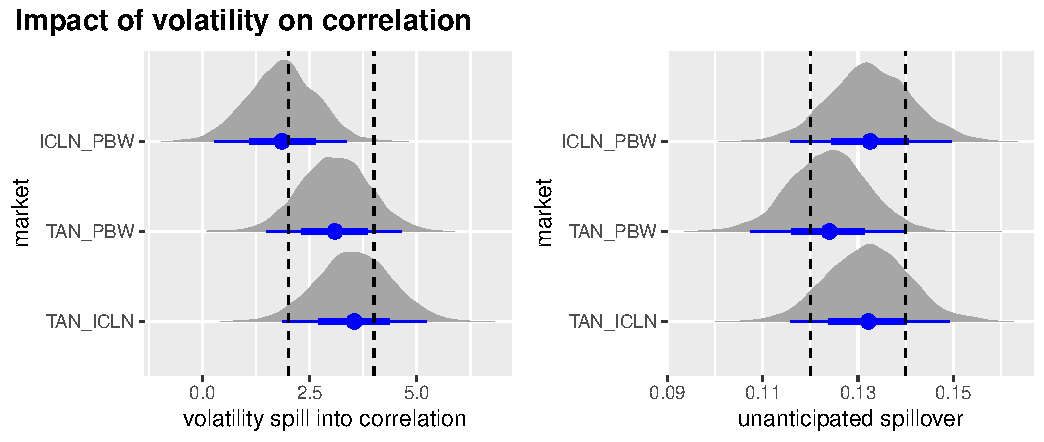
\includegraphics{compare.pdf}

To ground us in a more practical answer. We can say that a 10\% move
either in ICLN or PBW volatility will induce at least a 30\% in the
volatility of TAN, with moves as low as about 20\% and as high as about
45\%. A 10\% move in ICLN will induce a bit more than an 18\% move in
PBW, with moves as low as 6\% and as high as over 30\%. These intervals
are credible with 89\% probability.

Again we can review the role of each of the observations on the
bias-uncertainty tradeoff. High penalty-high \(k\) observations will
obscure efforts to predict correlations. The market to watch in this
regard is the ICLN-PBW pair, which coincides with the high volatilities
both of PBW and ICLN evident in the \(\sigma\) distributions we viewed
above.

\begin{Shaded}
\begin{Highlighting}[]
\DocumentationTok{\#\# R code 7.34 McElreath2020}
\CommentTok{\#library( plotly )}
\FunctionTok{options}\NormalTok{( }\AttributeTok{digits=}\DecValTok{2}\NormalTok{, }\AttributeTok{scipen=}\DecValTok{999999}\NormalTok{)}
\NormalTok{d }\OtherTok{\textless{}{-}}\NormalTok{ d\_4}
\FunctionTok{set.seed}\NormalTok{(}\DecValTok{4284}\NormalTok{)}
\NormalTok{m }\OtherTok{\textless{}{-}}\NormalTok{ m\_4}
\NormalTok{PSIS\_m }\OtherTok{\textless{}{-}} \FunctionTok{PSIS}\NormalTok{( m, }\AttributeTok{pointwise=}\ConstantTok{TRUE}\NormalTok{ )}
\NormalTok{PSIS\_m }\OtherTok{\textless{}{-}} \FunctionTok{cbind}\NormalTok{( PSIS\_m, }\AttributeTok{mid =}\NormalTok{ d}\SpecialCharTok{$}\NormalTok{markets )}
\FunctionTok{set.seed}\NormalTok{(}\DecValTok{4284}\NormalTok{)}
\CommentTok{\#WAIC\_m2.2 \textless{}{-} WAIC(m2.2,pointwise=TRUE)}
\NormalTok{p1 }\OtherTok{\textless{}{-}}\NormalTok{ PSIS\_m }\SpecialCharTok{\%\textgreater{}\%} 
  \FunctionTok{ggplot}\NormalTok{( }\FunctionTok{aes}\NormalTok{( }\AttributeTok{x=}\NormalTok{penalty, }\AttributeTok{y=}\NormalTok{k, }\AttributeTok{fill =}\NormalTok{ mid, }\AttributeTok{color =}\NormalTok{ mid ) ) }\SpecialCharTok{+}
  \FunctionTok{geom\_point}\NormalTok{( }\AttributeTok{shape=}\DecValTok{21}\NormalTok{ ) }\SpecialCharTok{+} 
  \FunctionTok{xlab}\NormalTok{(}\StringTok{"PSIS Pareto k"}\NormalTok{) }\SpecialCharTok{+} \FunctionTok{ylab}\NormalTok{(}\StringTok{"PSIS penalty"}\NormalTok{) }\SpecialCharTok{+} 
  \FunctionTok{geom\_vline}\NormalTok{( }\AttributeTok{xintercept =} \FloatTok{0.7}\NormalTok{, }\AttributeTok{linetype =} \StringTok{"dashed"}\NormalTok{) }\SpecialCharTok{+} 
  \FunctionTok{ggtitle}\NormalTok{( }\StringTok{"Market Spillover: "}\NormalTok{ )}
\NormalTok{p1 }\CommentTok{\#ggplotly( p1 )}
\end{Highlighting}
\end{Shaded}

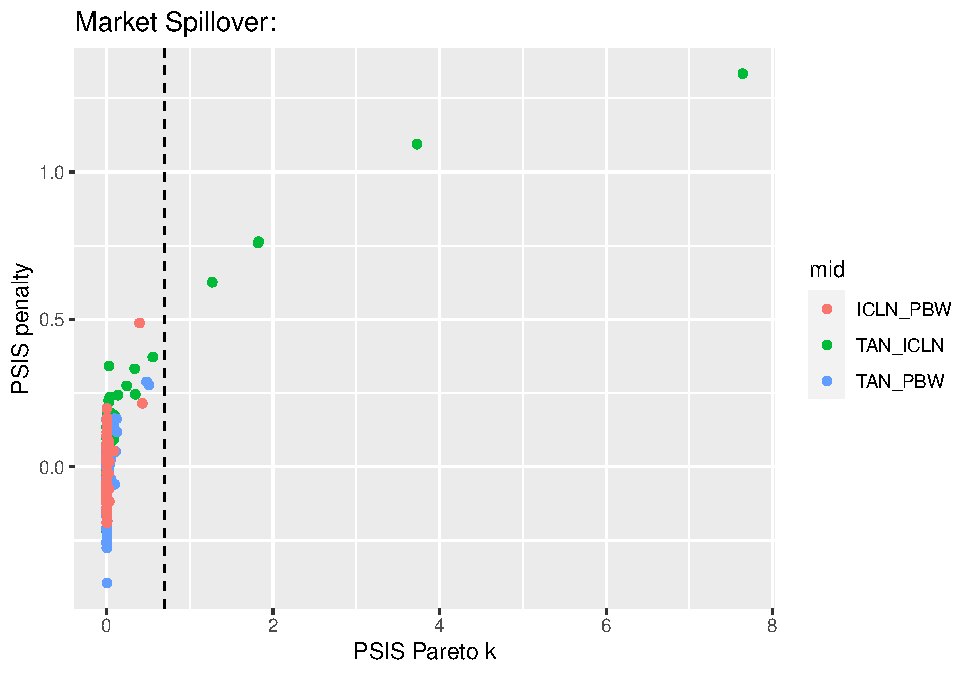
\includegraphics{market-facts_files/figure-latex/psis-spill-pbw-icln-1-1.pdf}
``` Most of the uncertainty is found in wind (PBW) volatility on solar
(TAN: green). The least uncertain market seems to be the relationship
between PBW and ICLN.

\hypertarget{what-have-we-accomplished}{%
\section{What have we accomplished?}\label{what-have-we-accomplished}}

We can provide provisional answers to the CFO's initial questions using
the work flows developed here.

\begin{itemize}
\item
  Univariate volatility clustering is compatible with highly kurtotis,
  and thus highly volatile volatility.
\item
  Volatile volatility in each asset spills into each market separately.
  These affects are measured using both quantile regression and Bayesian
  statistical techniques. The two approaches seem to agree on the
  probable existence of market spillover.
\item
  We tested the hypothesis that one market's riskiness affects
  another's, probably. They do, both in systematic, \(\beta\), and
  ideosyncratic, \(\sigma\), modes.
\item
  We find that a strongly coupled market risk structure persists across
  TAN, PBW and ICLN assets in each pair of market combinations.
\item
  TAN is the most sensitive market with highly volatile responses to
  ICLN and PBS volatility. Both ICLN and PBW are far less sensitive to
  moves within and across their markets.
\end{itemize}

The CFO should be wary that strong negative movements in one market will
probably persist and spill over into negative movements across the three
markets. Earnings based on this model will themselves exhibit the
results of volatility clustering and market spillover.

Our next step would be to build volatility clustering into a model to
derive implied capital requirements through market risk channels.

\hypertarget{references}{%
\section*{References}\label{references}}
\addcontentsline{toc}{section}{References}

\hypertarget{refs}{}
\begin{CSLReferences}{1}{0}
\leavevmode\hypertarget{ref-Carpenter2017}{}%
Carpenter, Gelman, B. 2017. {``Stan: A Probabilistic Programming
Language.''} \emph{Journal of Statistical Software} 76 (1).

\leavevmode\hypertarget{ref-Cont2001}{}%
Cont, R. 2001. {``Empirical Properties of Asset Returns: Stylized Facts
and Statistical Issues.''} \emph{Quantitative Finance} 1.

\leavevmode\hypertarget{ref-Embrechts2000}{}%
Embrechts, Haan, Paul. 2000. {``Modellinf Multivariate Extremes.''} In
\emph{Extremes and Integrated Risk Management}, edited by Paul
Embrechts, 59--67. RISK Publications.

\leavevmode\hypertarget{ref-GelmanHwangVehtari2013}{}%
Gelman, J. Hwang, A., and A. Vehtari. 2013. {``Understanding Predictive
Information Criteria for Bayesian Models.''}

\leavevmode\hypertarget{ref-Koenker2005}{}%
Koenker, Roger. 2005. \emph{Quantile Regression (Econometric Society
Monographs)}. Cambridge University Press.

\leavevmode\hypertarget{ref-McElreath2020}{}%
McElreath, Richard. 2020. \emph{Statistical Rethinking: {A Bayesian}
Course with Examples in {R} and {Stan}}. Second edition. {CRC Press}.
\url{https://xcelab.net/rm/statistical-rethinking/}.

\leavevmode\hypertarget{ref-mcneil2015quantitative}{}%
McNeil, A. J., R. Frey, and P. Embrechts. 2015. \emph{Quantitative Risk
Management: Concepts, Techniques and Tools - Revised Edition}. Princeton
Series in Finance. Princeton University Press.
\url{https://books.google.com/books?id=SfJnBgAAQBAJ}.

\leavevmode\hypertarget{ref-Orrell2020quantum}{}%
Orrell, D. 2020. \emph{Quantum Economics and Finance: An Applied
Mathematics Introduction}. Panda Ohana Publishing.
\url{https://books.google.com/books?id=OZaMzQEACAAJ}.

\leavevmode\hypertarget{ref-Taleb2018}{}%
Taleb, Nassim Nicholas. 2018. {``The Statistical Consequences of Fat
Tails: Papers and Commentary.''} Edited by Stem Academic Publishing.
\emph{The Technical Inconcerto} 1.

\leavevmode\hypertarget{ref-Stan2020a}{}%
Team, Stan Development. 2020a. {``RStan: The r Interface to Stan (r
Package Version 2.17.3) {[}Computer Software{]}.''}
\url{http://mc-stan.org/}.

\leavevmode\hypertarget{ref-Stan2020b}{}%
---------. 2020b. {``The Stan Core Library (Version 2.18.0).''}
\url{http://mc-stan.org/}.

\leavevmode\hypertarget{ref-VehtariGelmanGabry2015}{}%
Vehtari, A. Gelman, A., and J. Gabry. 2015. {``Efficient Implementation
of Leave-One-Out Cross-Validation and WAIC for Evaluating Fitted
Bayesian Models.''}

\end{CSLReferences}

\bibliographystyle{unsrt}
\bibliography{references.bib}


\end{document}
